%Metodología
\section{Metodología}\label{sec:metodologia}
\subsection{Parte 1. Aplicaciones De Las Topologías Clásicas}

\begin{figure}[H]
  \centering
  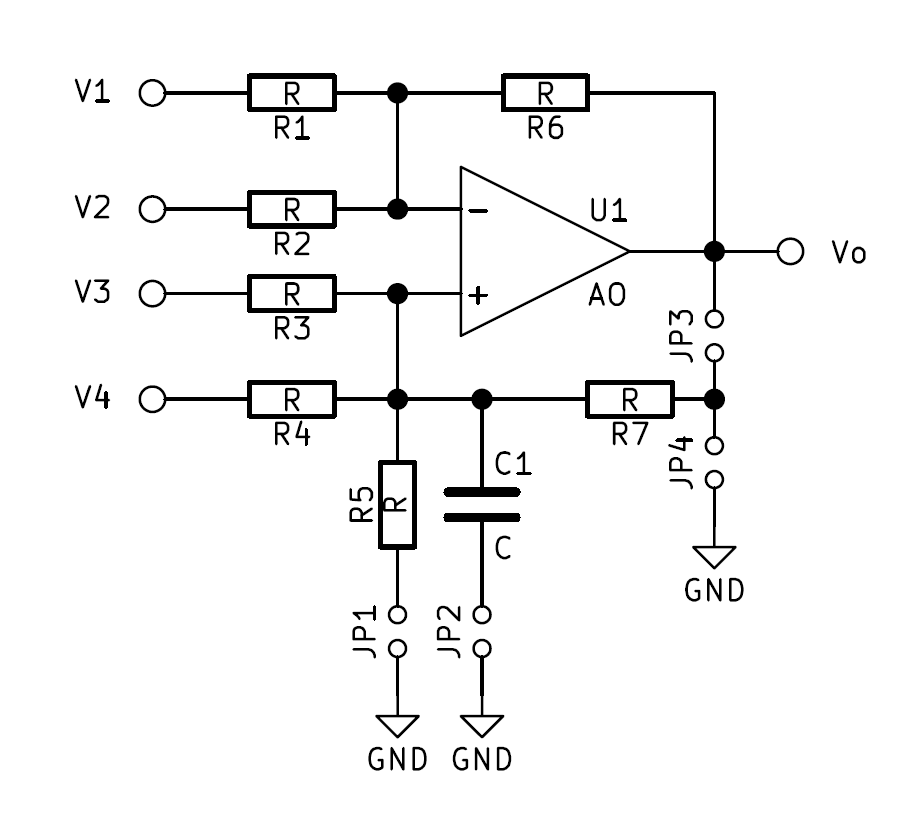
\includegraphics[width=8cm]{Imagenes/topologias_basicas.png}
  \caption{Topologías básicas}
  \label{fig:topologia_basicas}
\end{figure}

\begin{enumerate}[label=\textbf{\arabic*.}, font=\bfseries]
    
    \item Determinar la conexiones necesarias ($JP_j$: On/Off y señales de entrada $V_i$) para obtener un:

    \begin{itemize}
        \item \textbf{Amplificador Inversor}
            \begin{figure}[H]
              \centering              
              \includestandalone{Circuitos/inversor}
              \caption{Configuración del Amplificador Inversor}
              \label{fig:inversor}
            \end{figure}

        Si se observa la figura \ref{fig:topologia_basicas} de las topologías básicas, se obtiene un amplificador inversor con la siguiente configuración:

            \begin{itemize}
                \item  Entrada: $V_1$
                \item  $JP_1:$ On
                \item  $JP_2,JP_3,JP_4:$ Off
            \end{itemize}
        
        De esa manera, se obtiene la figura \ref{fig:inversor}
\newpage

        \item \textbf{Amplificador No Inversor}

            \begin{figure}[H]
              \centering              \includestandalone{Circuitos/no_inversor}
              \caption{Configuración del Amplificador No Inversor}
              \label{fig:no_inversor}
            \end{figure}
            
            Si se observa la figura \ref{fig:topologia_basicas} de las topologías básicas, se obtiene un amplificador no inversor con la siguiente configuración:

            \begin{itemize}
                \item  Entrada: $V_3$
                \item  Tierra: $V_1$
                \item  $JP_1, JP_2,JP_3,JP_4:$ Off
            \end{itemize}
        
        De esa manera, se obtiene la figura \ref{fig:no_inversor}
            

        \item \textbf{Amplificador Restador}

            \begin{figure}[H]
              \centering              \includestandalone{Circuitos/restador}
              \caption{Configuración del Amplificador Restador}
              \label{fig:restador}
            \end{figure}
            
            Si se observa la figura \ref{fig:topologia_basicas} de las topologías básicas, se obtiene un amplificador restador con la siguiente configuración:

            \begin{itemize}
                \item  Entrada: $V_1$ y $V_3$
                \item  $JP_1:$ On
                \item  $JP_2,JP_3,JP_4:$ Off
            \end{itemize}
        
        De esa manera, se obtiene la figura \ref{fig:restador}


        \textbf{Nota:} $V_1$ y $V_3$ realizan un corto para poder utilizar ambos nodos para la entrada del oscilador, obteniendo un $V_{osc}$

        \item \textbf{Convertidor de Tensión a Corriente (Fuente de Corriente)}

            \begin{figure}[H]
              \centering              \includestandalone{Circuitos/fuente_de_corriente}
              \caption{Configuración del Convertidor de Tensión a Corriente (Fuente de Corriente)}
              \label{fig:fuente_de_corriente}
            \end{figure}
            
            Si se observa la figura \ref{fig:topologia_basicas} de las topologías básicas, se obtiene un convertidor de fuente de tensión a corriente con la siguiente configuración:

            \begin{itemize}
                \item  Entrada: $V_4$
                \item  Tierra: $V_1$
                \item  $JP_1,JP_3:$ On
                \item  $JP_2,JP_4:$ Off
                \item  Carga: $R_5$
            \end{itemize}
        
        De esa manera, se obtiene la figura \ref{fig:fuente_de_corriente}

        \textbf{Nota:} Se conectará una fuente de voltaje de Corriente continua para observar como a través de su tensión podemos modificar la corriente.

\newpage
        \item \textbf{Integrador No Inversor (Integrador de Boo)}

            \begin{figure}[H]
              \centering              \includestandalone{Circuitos/integrador_no_inversor}
              \caption{Configuración del Integrador No Inversor}
              \label{fig:integrador_no_inversor}
            \end{figure}
            
            Si se observa la figura \ref{fig:topologia_basicas} de las topologías básicas, se obtiene un integrador no inversor con la siguiente configuración:

            \begin{itemize}
                \item  Entrada (Onda cuadrada): $V_4$ y @1KHz
                \item  Tierra: $V_1$
                \item  $JP_1,JP_3:$ On
                \item  $JP_2,JP_4:$ Off
                \item  Carga: $R_5$
            \end{itemize}
        
        De esa manera, se obtiene la figura \ref{fig:integrador_no_inversor}
        
    \end{itemize}
\subsubsection{Diseño y Simulación}

    \item Escoja los valores de las resistencias para obtener un Restador de ganancia 2, un inversor de ganancia -2, un amplificador No Inversor. Para el integrador utilice un condensador de poliéster de 10nF. Realice la simulación del circuito para verificar el resultado obtenido en sus cálculos. Explique cualquier diferencia respecto a sus cálculos, si la hay. Para probar la fuente de corriente, utilice diferentes valores de la resistencia de carga.
   
  % {\Large \textbf{Diseño}}
    \begin{itemize}
        \item \textbf{Inversor}

            \begin{equation}
                A_v=\dfrac{V_o}{V_i}=-\dfrac{R_6}{R_1}=-\dfrac{2K\ohm}{1K\ohm} = -2
                \label{eqn:A_inversor}
            \end{equation}

            \begin{itemize}
\newpage            
                \item Simulación

                    \begin{figure}[H]
                      \centering
                      \renewcommand{\figurename}{Gráfica}
                        \setcounter{figure}{0}
                      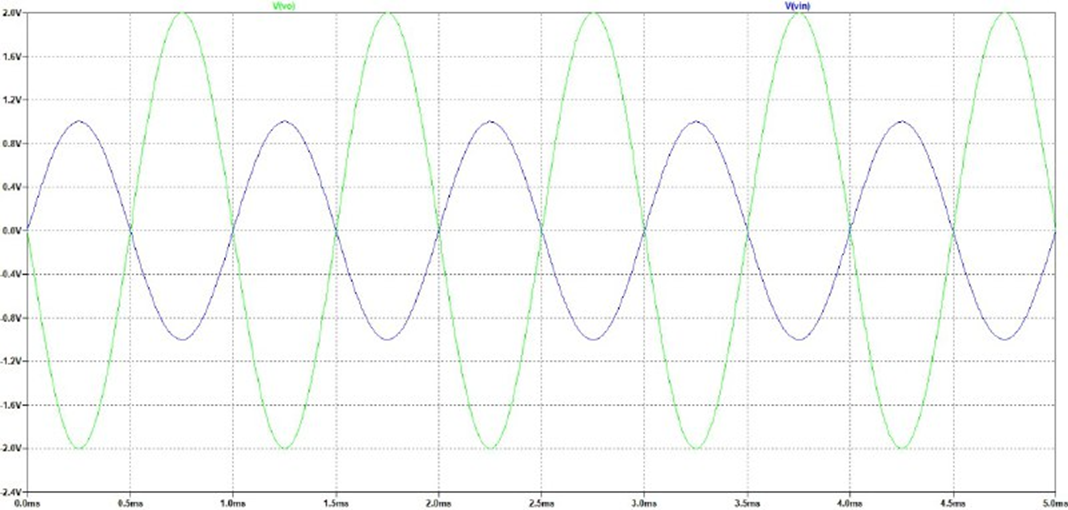
\includegraphics[width=\textwidth]{Imagenes/inversor.png}
                      \caption{Forma de ondas de la señal de salida y entrada de la figura \ref{fig:inversor}}
                      \label{fig:sim_inversor}
                    \end{figure}
            \end{itemize}

            Como Se puede observar en la gráfica \ref{fig:sim_inversor}, los cálculos de la ecuación \ref{eqn:A_inversor} concuerdan con la simulación.

        \item \textbf{No Inversor}

            \begin{align}
                A_v&=2=\dfrac{V_o}{V_i}=1+\dfrac{R_6}{R_1} \nonumber \\[0.2cm]
                2&=1+\dfrac{R_6}{R_1} \Longrightarrow 2-1=\dfrac{R_6}{R_1} \nonumber \\[0.8cm]
                R_1&=R_6=2K\ohm                     
                \label{eqn:A_no_inversor}
            \end{align}

\newpage                
            \begin{itemize}
                \item Simulación
                    \begin{figure}[H]
                      \centering
                      \renewcommand{\figurename}{Gráfica}
                      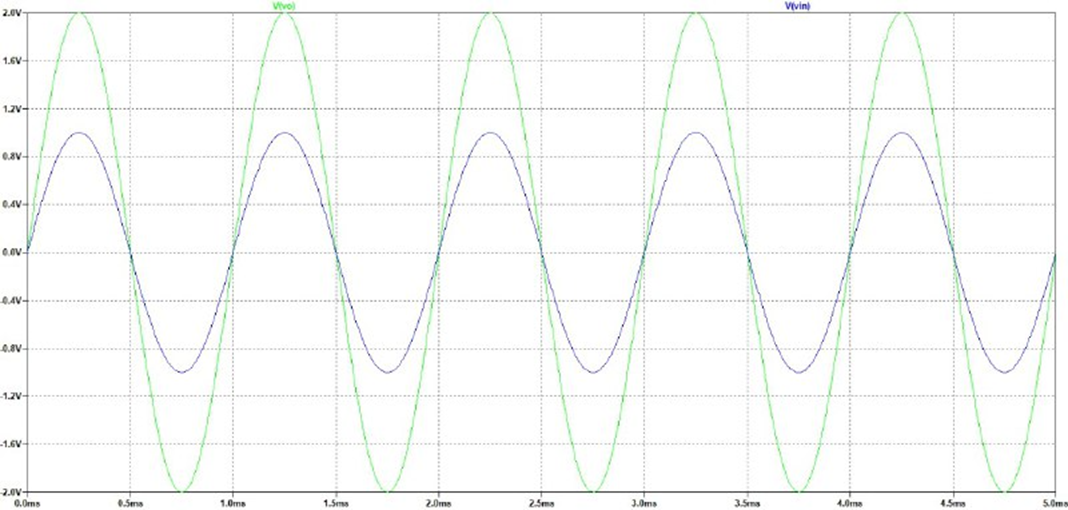
\includegraphics[width=\textwidth]{Imagenes/no_inversor.png}
                      \caption{Forma de ondas de la señal de salida y entrada de la figura \ref{fig:no_inversor}}
                      \label{fig:sim_no_inversor}
                    \end{figure}
            \end{itemize}

            Como Se puede observar en la gráfica \ref{fig:sim_no_inversor}, el diseño que se realizo fue el adecuado debido a que  concuerdan con la simulación.
            
            \textbf{Nota:} El máximo voltaje de entrada es de $4V$ debido a que su ganancia es 2, su $V_o=8V$ despues de $8V$ se satura su salida.

        \item \textbf{Restador}

            Se toma en consideración que si se observa el nodo no inversor de la figura \ref{fig:restador}, siendo este un divisor de tensión se tiene un no inversor y de esta manera se puede hallar su ganancia, debido a esto se realizará una superposición para hallar la ganancia de ambas, de esa manera se tiene un inversor y un no inversor al "apagar" las fuentes de tensión aplicando lo anteriormente mencionado.

            \begin{gather}
                V_o=-\dfrac{R_6}{R_1}V_1+\dfrac{R_5}{R_5+R_3}V_3\left(1+\dfrac{R_6}{R_1}\right)\label{eqn:vo}\\[0.2cm]
                \dfrac{R_6}{R_1}=1 \Longrightarrow R_6=R_1 \label{eqn:1} \\[0.2cm] 
                \dfrac{R_5}{R_5+R_3}V_3 \left(1+\dfrac{R_6}{R_1}\right)=3
                \label{eqn:2}   
            \end{gather}

            Ahora se toma la ecuación \ref{eqn:1} en la ecuación \ref{eqn:2}, teniendo a continuación lo siguiente:

            \begin{gather}
                \dfrac{R_5}{R_5+R_3}V_3 \left(1+\dfrac{R_6}{R_1}\right)=3 \nonumber\\[0.5cm]
                \dfrac{R_5}{R_5+R_3}V_3 \left(1+\dfrac{R_1}{R_1}\right)=3 \Longrightarrow 2R_5=3R_3+3R_5 \nonumber\\[0.5cm]
                -3R_3=3R_5-2R_5 \nonumber\\[0.5cm]
                |-3R_3=R_5| \Longrightarrow R_5=3R_3 \label{eqn:3}           
            \end{gather}

            Por lo tanto, se tiene que el voltaje de salida $V_o$ de la ecuación \ref{eqn:vo} se le van a sustituir las ecuaciones \ref{eqn:1} y \ref{eqn:3}, obteniendo lo siguiente:

            \begin{gather}
                V_o=-V_1+\dfrac{-3R_3}{R_3-3R_3}(1+1)V_3=-V_1+3V_3 \label{eqn:vo_1}
            \end{gather}

            Se tiene la ecuación \ref{eqn:vo_1}, y sabiendo que $V_i=V_1=V_3$ se sustituye en la ecuación antes nombrada dando como resultado,

            \begin{gather}
                V_o=-V_i+3V_i \nonumber \\[0.5cm]
                \dfrac{V_o}{V_i}=2 \nonumber
            \end{gather}

            \begin{itemize}
                \item Simulación
                
                    Se unen las entradas debido a que no tenemos otra salida de voltaje de entrada en el laboratorio por esa razón lo colocamos como si fuese un común.

                    \begin{figure}[H]
                      \centering
                      \renewcommand{\figurename}{Gráfica}
                      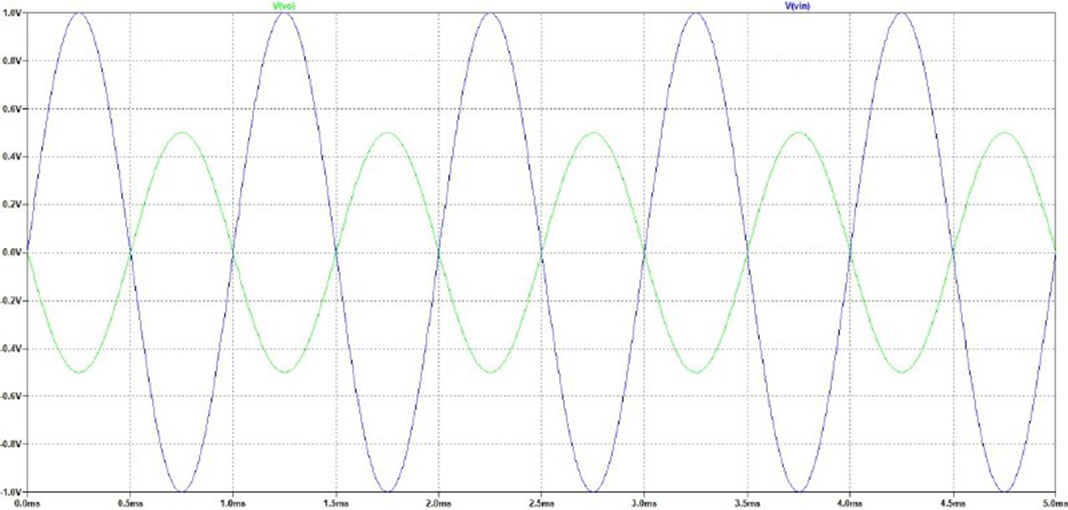
\includegraphics[width=\textwidth]{Imagenes/restador.png}
                      \caption{Forma de ondas de la señal de salida y entrada de la figura \ref{fig:restador}}
                      \label{fig:sim_restador}
                    \end{figure}
            \end{itemize}
        \item \textbf{Convertidor de Tensión a Corriente (Fuente de Corriente)}

            \begin{figure}[H]
              \centering
              \renewcommand{\figurename}{Imagen}
              \setcounter{figure}{0}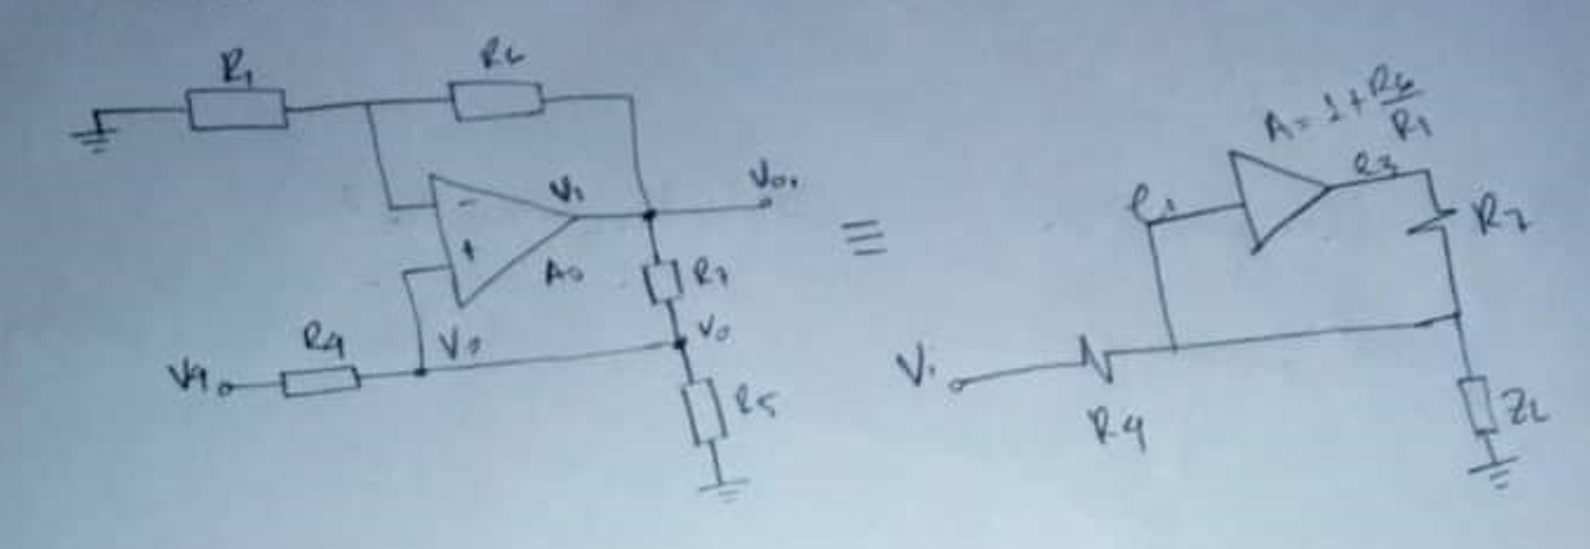
\includegraphics[width=\textwidth]{Imagenes/fuente.png}
              \caption*{}
              \label{fig:fuente}
            \end{figure}
            \begin{figure}[H]
              \centering
              \renewcommand{\figurename}{Imagen}
              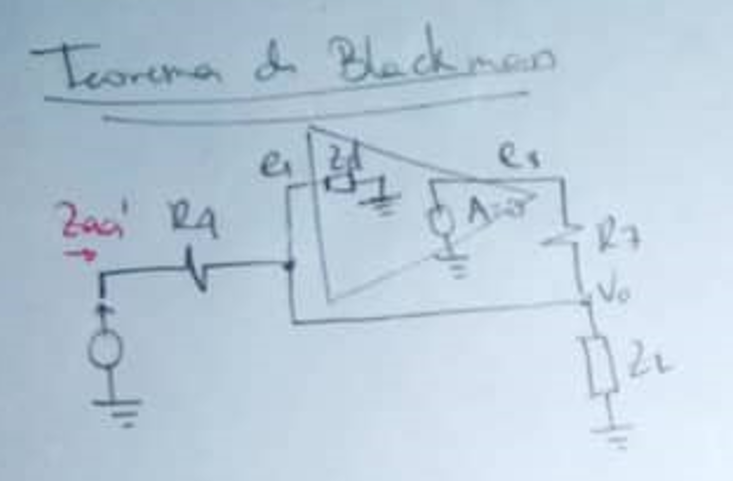
\includegraphics[width=10cm]{Imagenes/fuente_2.png}
              \caption{Imagen de simplificación del circuito aplicando la Teorema de Blackman}
              \label{fig:fuente2}
            \end{figure}

            Por ser una fuente de corriente se tiene que la impedancia $Z_a\to \infty$, por esa razón se tiene lo siguiente:

            \begin{gather}
                Z_{aa'}=R_7//R_4 \label{eqn:zaa}\\[0.5cm]
                X_{31CC}=0 \label{eqn:x31cc}\\[0.5cm]
                X_{31CA}=R4 \label{eqn:x31ca}
            \end{gather}

            Haciendo uso de las ecuaciones \ref{eqn:zaa}, \ref{eqn:x31cc} y \ref{eqn:x31ca}, usando el teorema de Blackman se obtiene,

            \begin{gather}
                z_a=Z_{aa}\dfrac{1-AX_{31CC}}{1-AX_{31CA}} \nonumber\\[0.5cm]
                z_a=\dfrac{R_7R_4}{R_7+R_4}\dfrac{1-\left(1+\dfrac{R_6}{R_1}\right)(0)}{1-\left(1-\dfrac{R_6}{R_1}\right)R_4} \label{eqn:za}\\[0.5cm]
                R_7+R_4=R_4\left(1+\dfrac{R_6}{R_1}\right)=R_4\left(\dfrac{R_1+R_6}{R_1}\right) \nonumber\\[0.5cm]
                R_1(R_7+R_4)=R_4(R_1+R_6) \nonumber\\[0.5cm]
                R_1=R_4 \label{eqn:r1}\\[0.5cm]
                (R_7+R_4)=(R_1+R_6) \label{eqn:r7}\\[0.5cm]
                \text{Haciendo uso de la ecuación \ref{eqn:r1} la sustituimos en \ref{eqn:r7}}\nonumber\\[0.5cm]
                R_7=R_6\\[0.5cm]
                R_1=R_4=10k\ohm \nonumber\\[0.5cm]
                R_7=R_6=4k\ohm \nonumber
            \end{gather}

            \begin{figure}[H]
              \centering
              \renewcommand{\figurename}{Imagen}
              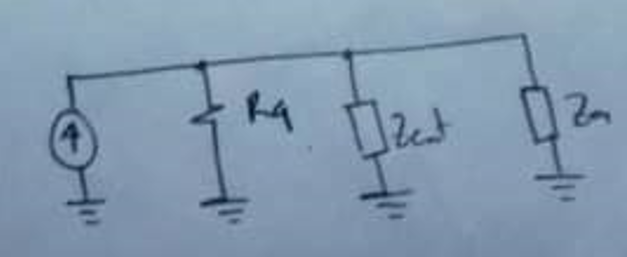
\includegraphics[width=10cm]{Imagenes/fuente_eq.png}
              \caption{Circuito equivalente de la fuente de corriente}
              \label{fig:fuenteeq}
            \end{figure}

            Por ley de ohm se tiene que $V_1=I_1R_4$ por lo tanto si se despeja $I=1mA$

            Por lo tanto, $V_o=R_LI_1=4K(1mA)=4V$
                
            \begin{itemize}
                \item Simulación

                    \begin{figure}[H]
                      \centering
                      \renewcommand{\figurename}{Gráfica}
                      \setcounter{figure}{3}
                      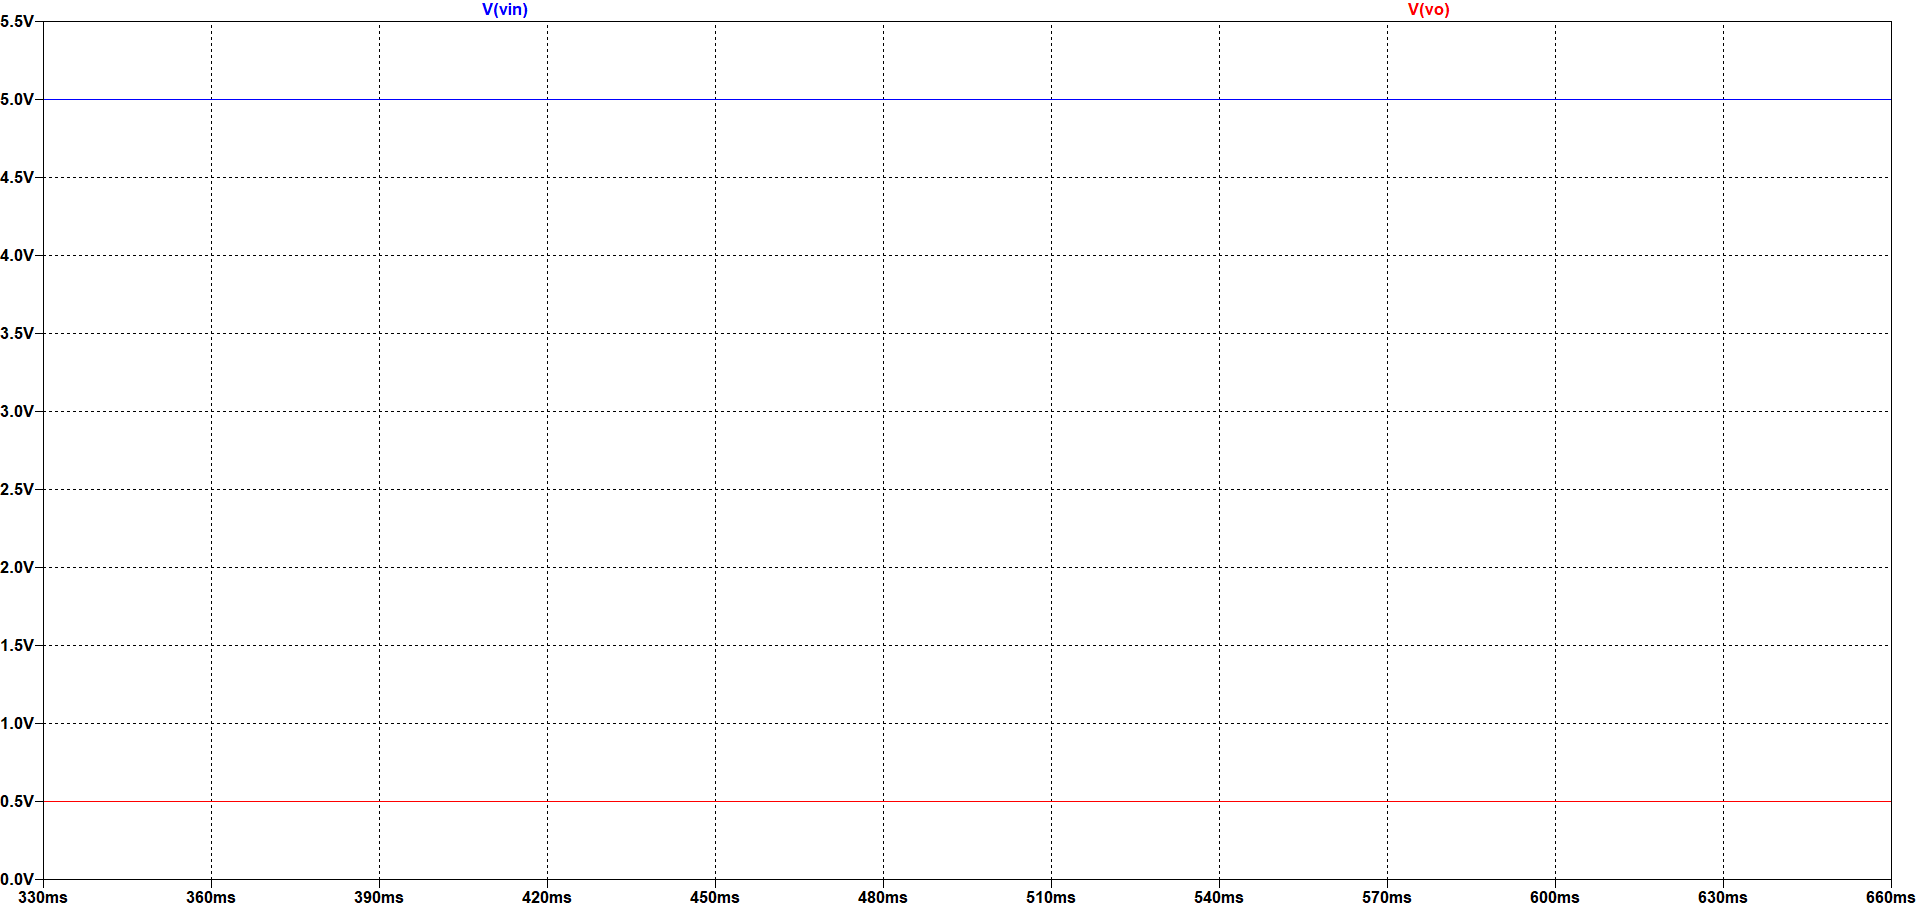
\includegraphics[width=\textwidth]{Imagenes/sim_fuente.png}
                      \caption{Forma de ondas de la señal de salida y entrada de la figura \ref{fig:fuente_de_corriente} con $R_L=1k$; Vo=0.5V; Io=0.5mA.}
                      \label{fig:sim_fuente}
                    \end{figure}
                    \begin{figure}[H]
                      \centering
                      \renewcommand{\figurename}{Gráfica}
                      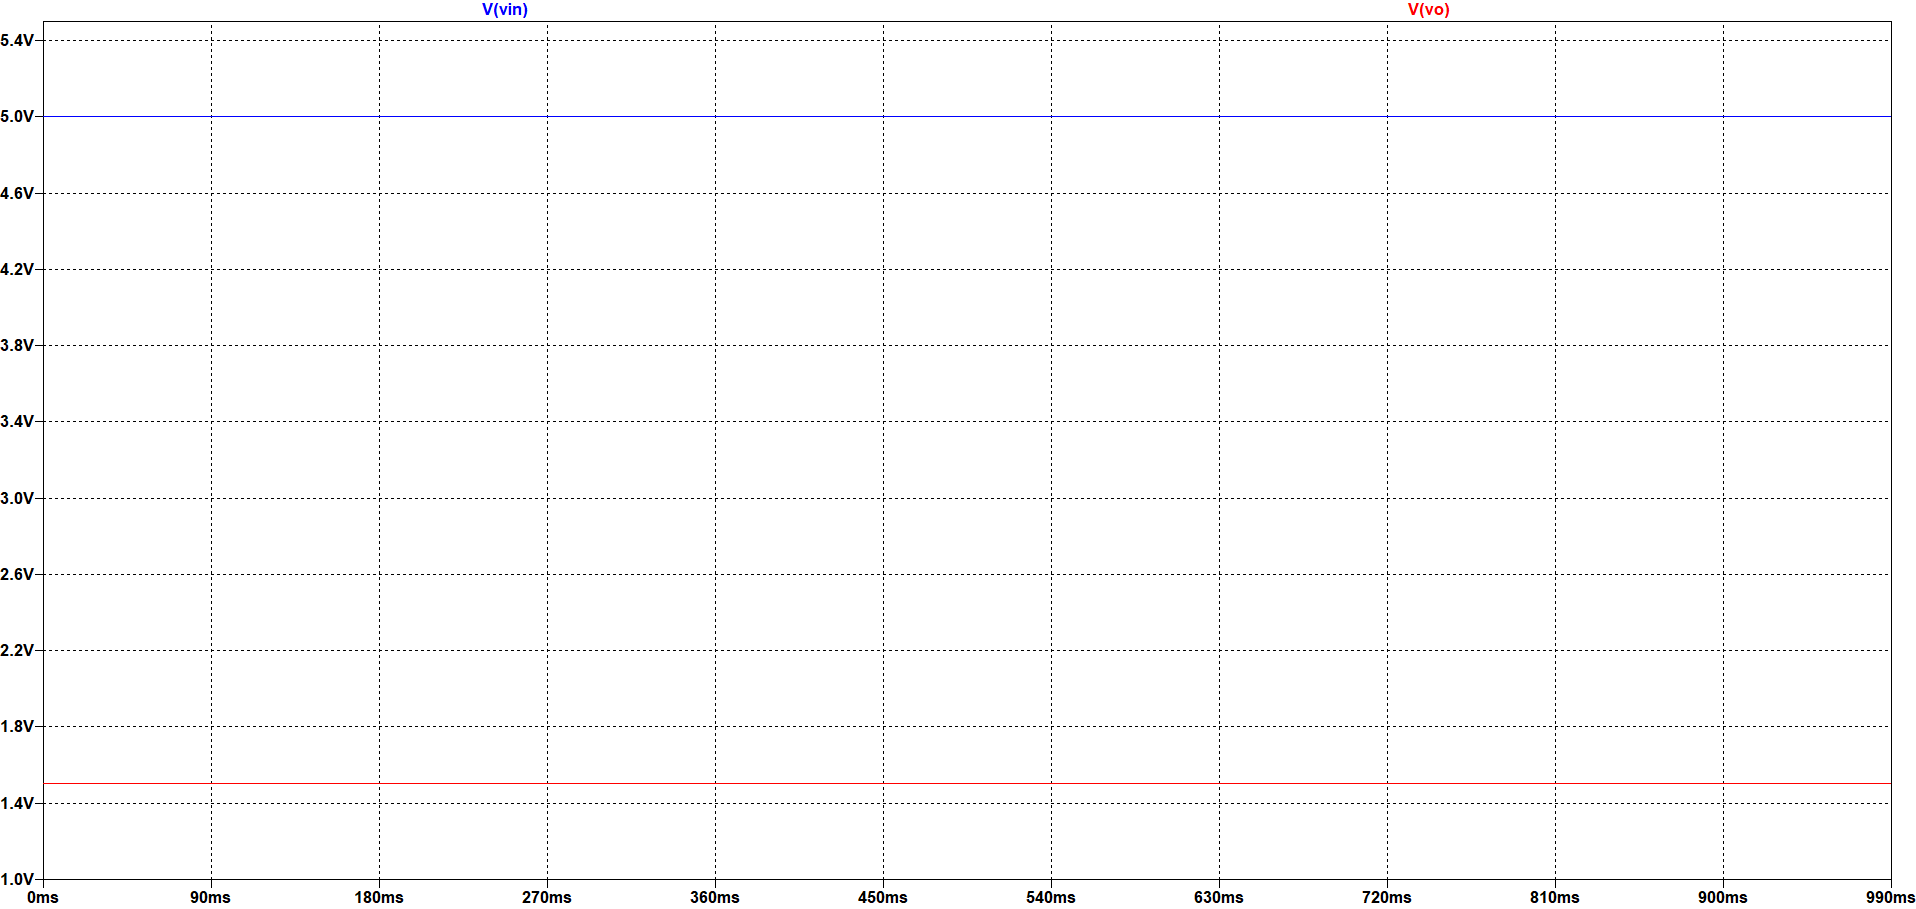
\includegraphics[width=\textwidth]{Imagenes/sim_fuente2.png}
                      \caption{Forma de ondas de la señal de salida y entrada de la figura \ref{fig:fuente_de_corriente} con $R_L=3k$; Vo=1.5V; Io=0.5mA.}
                      \label{fig:sim_fuente2}
                    \end{figure}

                    Se mantuvo la corriente y vario el voltaje de salida, como se observa en los cálculos realizados.

                    \begin{figure}[H]
                      \centering
                      \renewcommand{\figurename}{Gráfica}
                      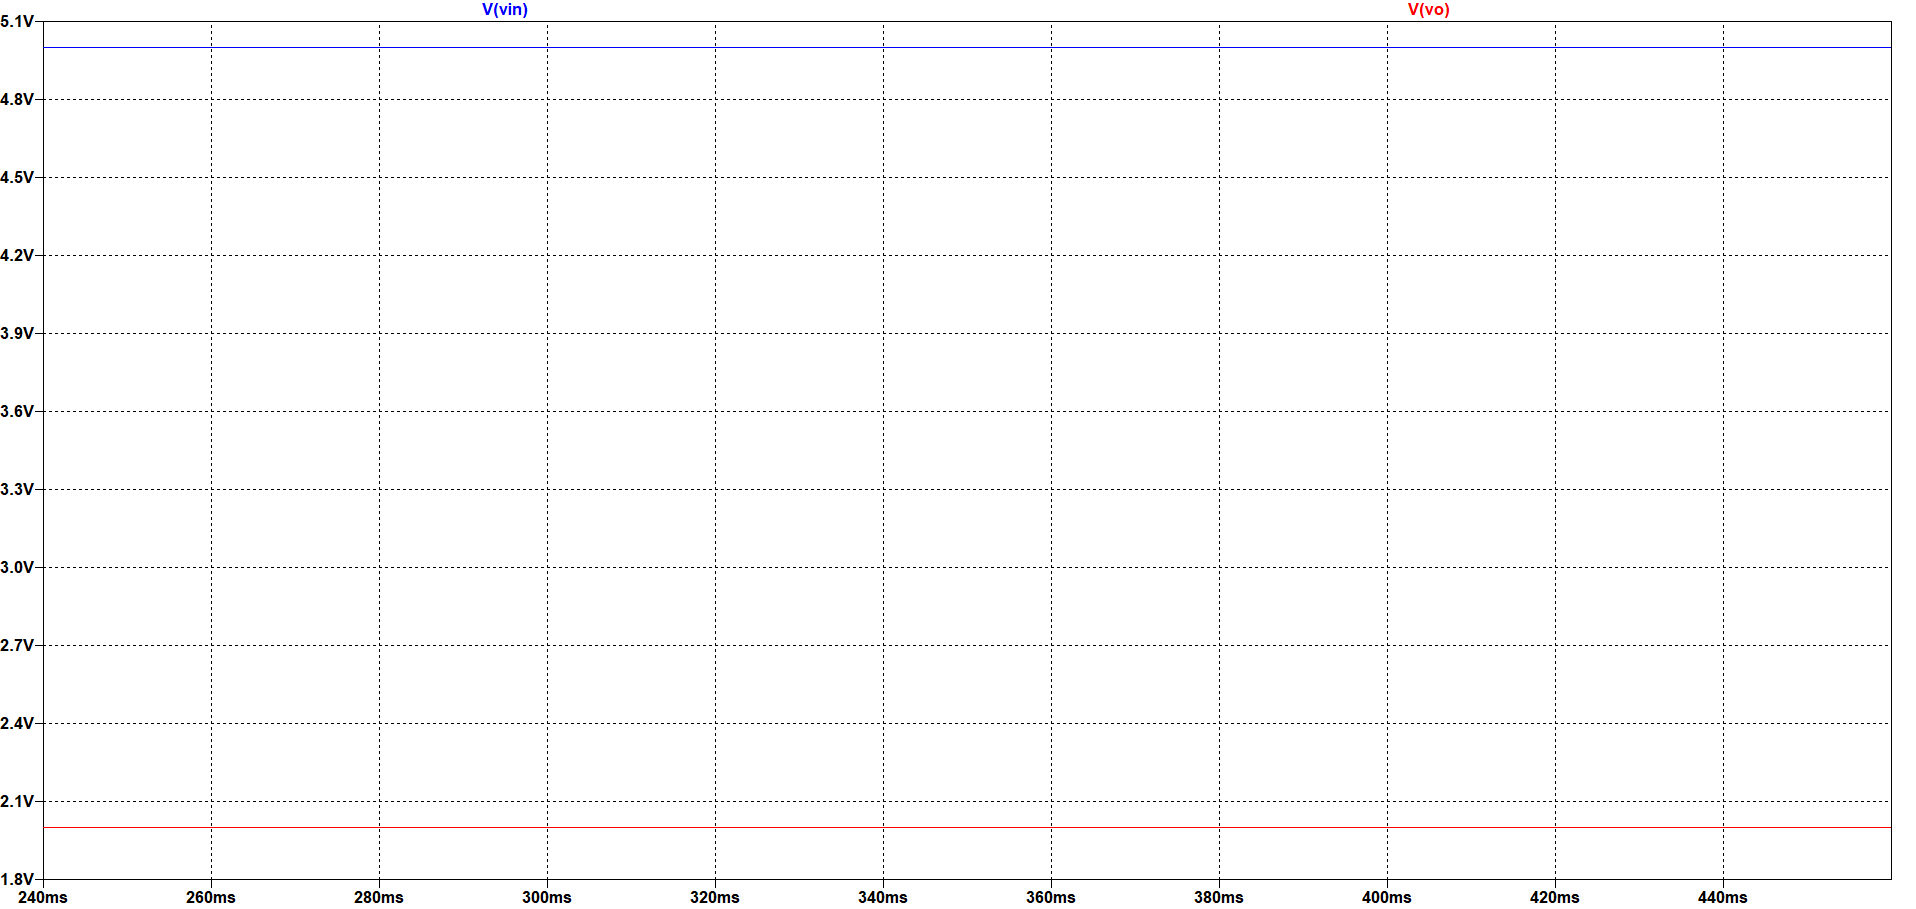
\includegraphics[width=\textwidth]{Imagenes/sim_fuente3.png}
                      \caption{Forma de ondas de la señal de salida y entrada de la figura \ref{fig:fuente_de_corriente} con $R_L=4k$; Vo=2V; Io=0.5mA.}
                      \label{fig:sim_fuente3}
                    \end{figure}

                    Solo Vario $V_o$

                    \begin{figure}[H]
                      \centering
                      \renewcommand{\figurename}{Gráfica}
                      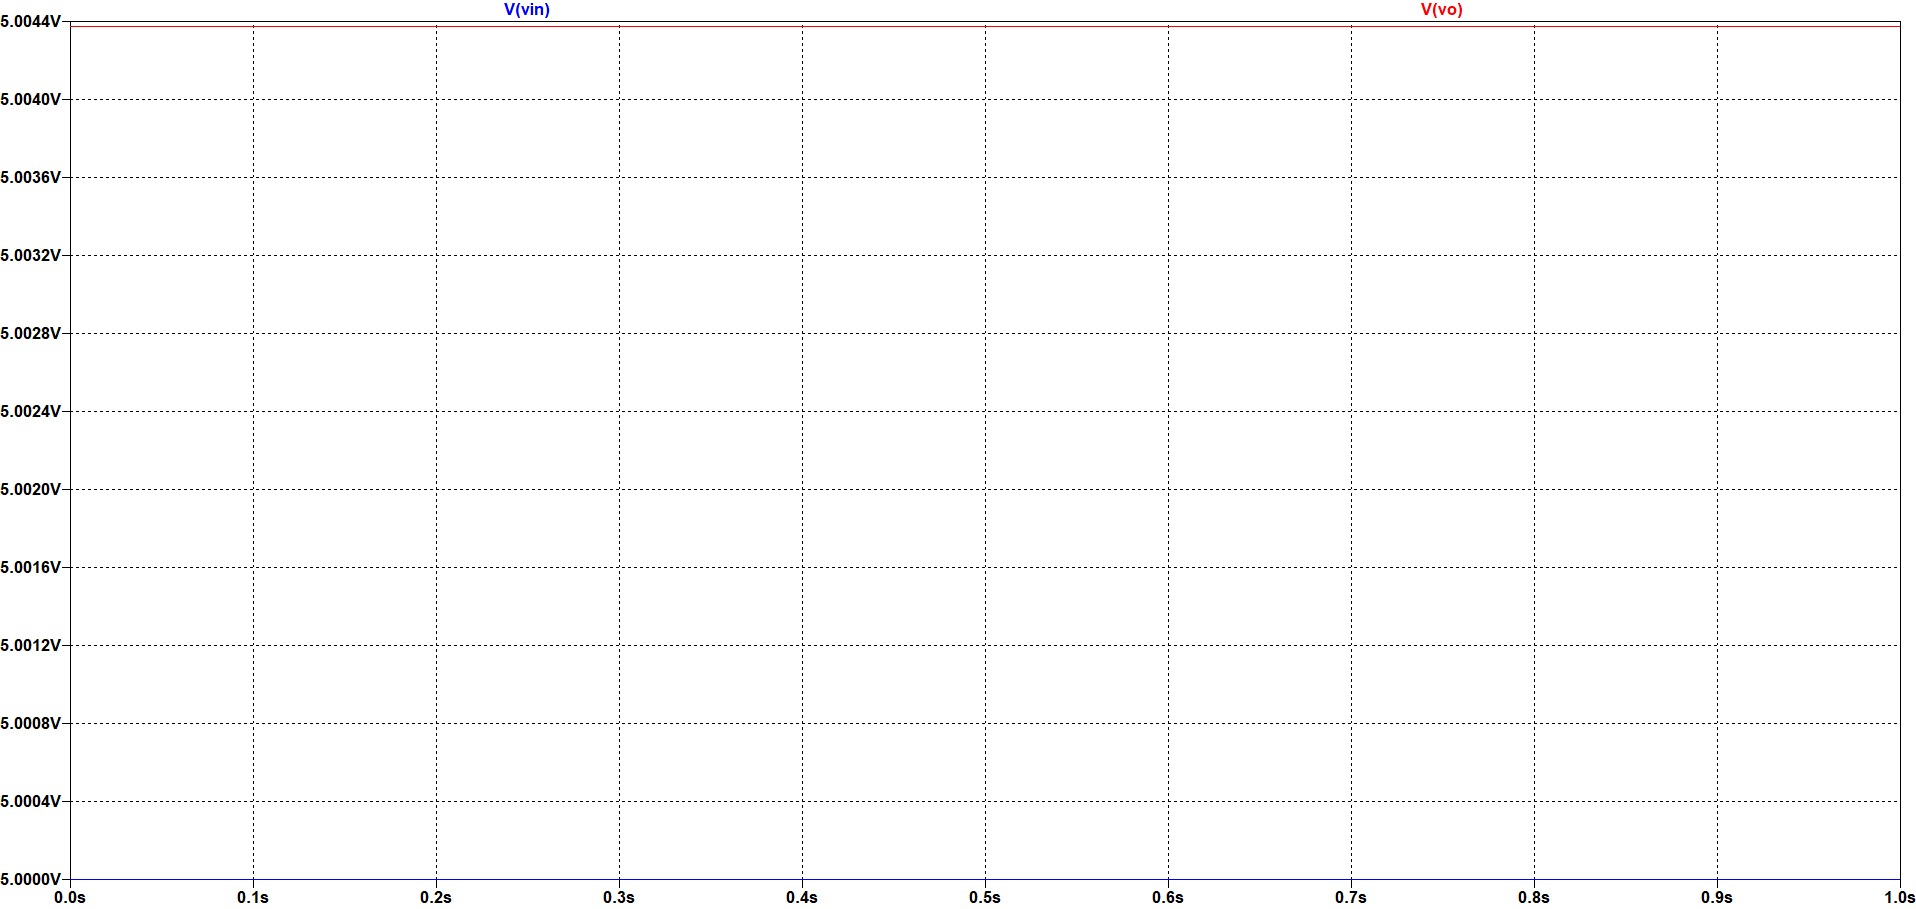
\includegraphics[width=\textwidth]{Imagenes/sim_fuente4.png}
                      \caption{Forma de ondas de la señal de salida y entrada de la figura \ref{fig:fuente_de_corriente} con $R_L=10k$; Vo=5.004V; Io=0.5mA.}
                      \label{fig:sim_fuente4}
                    \end{figure}

                    $V_o$ aumento pero su corriente no sobre pasa el $1mA$, solo disminuye un poco.
            \end{itemize}
        \item \textbf{Integrador No Inversor (Integrador de Boo)}
            En este caso, en el voltaje de entrada va a ser una onda cuadrada para poder observar el voltaje de salida necesario, haciendo uso de la siguiente ecuación:

            \begin{gather}
                V_{o'}=\left(1+\dfrac{R_6}{R_1}\right)V_o \nonumber\\[0.5cm]
                V_{o'}=\left(\dfrac{R_1+R_6}{R_1}\right)\dfrac{1}{R_4}\dfrac{1}{2CS}V_i \nonumber\\[0.5cm]
                \dfrac{V_{o'}}{V_i}=H(s)=\dfrac{R_1+R_6}{R_1R_42CS}\quad \therefore \nonumber\\[0.5cm]
                \dfrac{V_o}{V_i}=\dfrac{1}{R_42CS} \label{eqn:H}\\[0.5cm]
                Z_{load}=\dfrac{1}{2CS}
            \end{gather}

            \begin{itemize}
                \item Simulación
                    \begin{figure}[H]
                      \centering
                      \renewcommand{\figurename}{Gráfica}
                      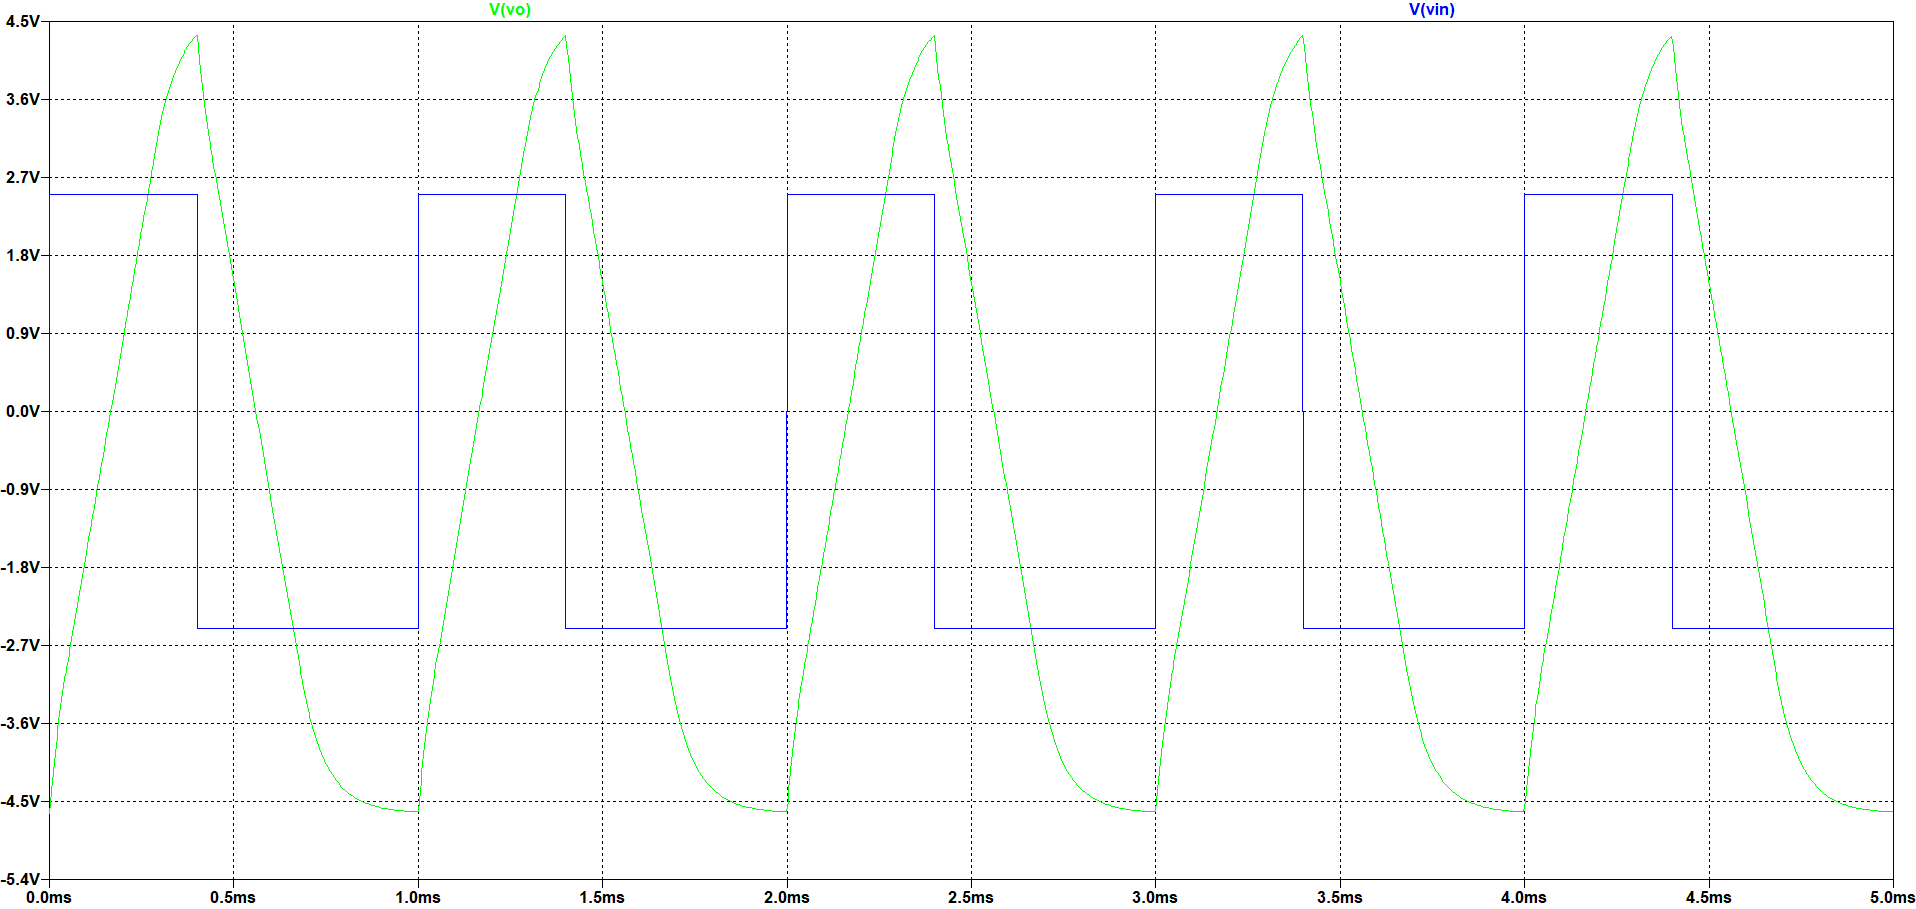
\includegraphics[width=\textwidth]{Imagenes/sim_intnoinver.png}
                      \caption{Forma de ondas de la señal de salida y entrada de la figura \ref{fig:integrador_no_inversor}}
                      \label{fig:sim_intnoinv}
                    \end{figure}

                    Se mantiene la configuración de las resistencias del circuito anterior, diferencia una señal cuadrada o un pulso de 10V
            \end{itemize}
    \end{itemize}
\end{enumerate}

\subsection{Parte 2. Amplificador Operacional Real}


\begin{table}[H]
    \centering
    \begin{tabular}{|c|c|}
        \hline
        \textbf{Componente} & \textbf{Valor} \\\hline
        $\mathbf{R_1}$ &  $100\si{\ohm}$ \\\hline
        $\mathbf{R_2}$ & $100 \si{\ohm}$  \\\hline
        $\mathbf{R_3}$ & $22 M \si{\ohm}$  \\\hline
        $\mathbf{R_4}$ & $22 M \si{\ohm}$   \\\hline
        $\mathbf{R_5}$ & $100k\si{\ohm}$  \\\hline
        $\mathbf{R_6}$  & $10k\si{\ohm}$ \\\hline
        $\mathbf{R_7}$  & $1k\si{\ohm}$ \\\hline
        $\mathbf{R_8}$  & $910\si{\ohm}$ \\\hline
        $\mathbf{R_9}$  & $10k\si{\ohm}$ \\\hline
        $\mathbf{R_{10}}$  & $91k\si{\ohm}$ \\\hline
        $\mathbf{R_v}$  & $1\approx 10 \si{\ohm}$ \\\hline
        $\mathbf{C}$  & $100 nF$ \\\hline
    \end{tabular}
    \caption{Lista de Componentes usados en el laboratorio n°2 de la Práctica n°2}
    \label{tab:componentes_1}
\end{table}

\begin{enumerate}[label=\textbf{\arabic*.}, font=\bfseries]
    \begin{figure}[H]
      \centering
      \setcounter{figure}{22}
      \includestandalone{Circuitos/AmplificadorReal}
      \caption{Medición de tensiones de Offset y corriente de polarización}
      \label{fig:amp_op_real}
    \end{figure}
    
    \item Haciendo uso del montaje indicado en el diagrama esquemático de la Figura \ref{fig:amp_op_real} explicar como medir la tensión de Offset y como medir la corriente de polarización de cada entrada.

    \begin{enumerate}
        \item Tensión Offset
        
            Para hallar la \textbf{tensión offset}, denotada como $V_{os}$, se va a cerrar los \textbf{Jumper(JP) 1 y 2}, de esa manera se obtiene la siguiente expresión:
            \begin{align*}
                V_{o} = \frac{R_{5}}{R_{2}}V_{os}    
            \end{align*}
        
            Se medirá la tensión de salida $V_o$, por esa razón, se despeja $V_{os}$, obteniendo de manera indirecta la \textbf{tensión offset}.
            \begin{equation}
                V_{os}=\dfrac{V_o}{1+\dfrac{R_5}{R_2}}
                \label{eqn:vos}
            \end{equation}

        \item Corriente de polarización 1
            Para hallar la \textbf{Corriente de polarización 1}, denotada como $I_{B_1}$, se cierra \textbf{JP 2} y se abre \textbf{JP 1}.
            \textbf{Nota:} Importante acotación para facilitar los cálculos es que la resistencia $R_1$ no se tomará en cuenta su caída de tensión, debido a que la corriente que pasa por allí es muy pequeña, en consecuencia se desprecia esa tensión. Por lo tanto, se obtiene lo siguiente:

            \begin{align*}
                V_{o} = (V_{os}-I_{B_1}R_3)\left(1+\dfrac{R_5}{R_2}\right)      
            \end{align*}

            Se medirá la tensión de salida $V_o$. Teniendo todos los demás datos exceptuando $I_{B_1}$, es la que se despejará, resultando la siguiente ecuación:

            \begin{equation}
                I_{B_1}=\dfrac{V_{os}\left(1+\dfrac{R_5}{R_2}\right)-V_o}{R_3\left(1+\dfrac{R_5}{R_2}\right)}
                \label{eqn:ib1}
            \end{equation}

            Se halla así la corriente de polarización 1, en la medición indirecta de la ecuación \ref{eqn:ib1}.

        \item Corriente de polarización 2

            Para hallar la \textbf{Corriente de polarización 2}, denotada como $I_{B_2}$, se cierra \textbf{JP 1} y se abre \textbf{JP 2}. Se toma en cuenta la nota anterior, se obtiene:

             \begin{align*}
                V_{o} = (V_{os}+I_{B_2}R_3)\left(1+\dfrac{R_5}{R_2}\right)      
            \end{align*}

            Se medirá la tensión de salida $V_o$. Teniendo todos los demás datos exceptuando $I_{B_2}$, es la que se despejará, resultando la siguiente ecuación:

            \begin{equation}
                I_{B_2}=\dfrac{V_o-V_{os}\left(1+\dfrac{R_5}{R_2}\right)}{R_4\left(1+\dfrac{R_5}{R_2}\right)}
                \label{eqn:ib2}
            \end{equation}

            Se halla así la corriente de polarización 2, en la medición indirecta de la ecuación \ref{eqn:ib2}.

        \item Corriente Offset

            Al hallar las corrientes de polarización de cada entrada, se puede hacer uso de la siguiente ecuación para conocer la \textbf{Corriente offset}

            \begin{equation}
                I_{os}=\left|I_{B_1}-I_{B_2}\right|
                \label{eqn:ios}
            \end{equation}
            
    \end{enumerate}

    \begin{figure}[H]
      \centering
      \includestandalone{Circuitos/GBWP}
      \caption{Medición del GBWP}
      \label{fig:GBWP}
    \end{figure}

    \item Mediante el montaje de la Figura \ref{fig:GBWP} explique como comprobar que el Producto del Ancho de Banda por la Ganancia (GBWP) se mantiene.

        En este caso, se verificará que con distintas configuraciones de la figura \ref{fig:GBWP}, se mantiene el GBWP, midiendo de manera experimental su frecuencia de corte en las distintas topologías (variando su frecuencia y observar su atenuación) y poder aproximar su respuesta en frecuencia.

        \textbf{Nota:} El producto de ancho de banda por ganancia, también conocido como producto ganancia-ancho de banda (GBWP), es un parámetro importante en el diseño de amplificadores operacionales. Se define como el producto de la ganancia de lazo cerrado por la banda de frecuencias. Este producto es una constante, lo que significa que si la ganancia disminuye, el ancho de banda aumenta, y viceversa.
        En el contexto de los amplificadores operacionales, el GBWP es crucial, ya que indica la relación inversa entre la ganancia y el ancho de banda. Un amplificador operacional sin realimentar tiene una ganancia considerable y un ancho de banda muy reducido. A partir de la frecuencia de corte, hay una caída de ganancia con una pendiente específica.

        \begin{itemize}
            \item \textbf{JP3 y JP4 abiertos}

                \begin{equation}
                    A_{2} = 1+ \frac{R_{10}+R_{9}}{R_{7}} = 102
                    \label{eqn:A2}
                \end{equation}

                Recordar que la primera ganancia es la que se obtiene en la frecuencia mas baja.

            \item \textbf{JP4 cerrado y JP3 abierto}

                \begin{equation}
                    A_{3} = 1+ \frac{R_{9}}{R_{7}} = 11
                    \label{eqn:A3}
                \end{equation}

            \item \textbf{JP4 y JP3 cerrados (Buffer)}

                \begin{equation}
                    A_{4} = 1 
                    \label{eqn:A4}
                \end{equation}

        \end{itemize}

    

    \begin{figure}[H]
      \centering
      \includestandalone{Circuitos/buffer}
      \caption{Medición de S.R., excursión máxima y corriente de corto circuito}
      \label{fig:buffer}
    \end{figure}

    \item Mediante el montaje de seguidor de tensión de la Figura \ref{fig:buffer}, indique como medir el Slew Rate (S.R. o tasa de variación en español), los limites máximos de excursión y la corriente de corto circuito.

        \begin{itemize}
            \item Slew Rate

                Antes de realizar el experimento colocar una frecuencia de 1KHz para luego poder realizar las variaciones. Se realizará con las siguientes instrucciones:
    
                Para medir el slew rate utilizando un osciloscopio, se debe conectar el osciloscopio a la salida del amplificador y configurarlo para mostrar la forma de onda de la señal de salida. Luego, se debe aplicar una señal de entrada triangular al amplificador y ajustar la frecuencia de la señal para que esté dentro del rango de operación del amplificador. A continuación, se debe medir el tiempo que tarda la señal de salida en cambiar desde el 10\% al 90\% de su valor máximo, y utilizar esta información para calcular el slew rate utilizando la siguiente fórmula:
                
                \begin{gather}
                    SR= \dfrac{\vartriangle V}{\vartriangle t} \label{eqn:sr}
                \end{gather}
     
                Donde SR es el slew rate, $\vartriangle V$ es el cambio en la tensión de salida y $\vartriangle t$ es el tiempo que tarda la señal de salida en cambiar desde el 10\% al 90\% de su valor máximo. Es importante tener en cuenta que el slew rate puede variar dependiendo de la frecuencia de la señal de entrada, por lo que se deben realizar mediciones en diferentes frecuencias para obtener una medida precisa del slew rate.
    
                \begin{figure}[H]
                  \centering
                  \renewcommand{\figurename}{Imagen}
                  \setcounter{figure}{2}
                  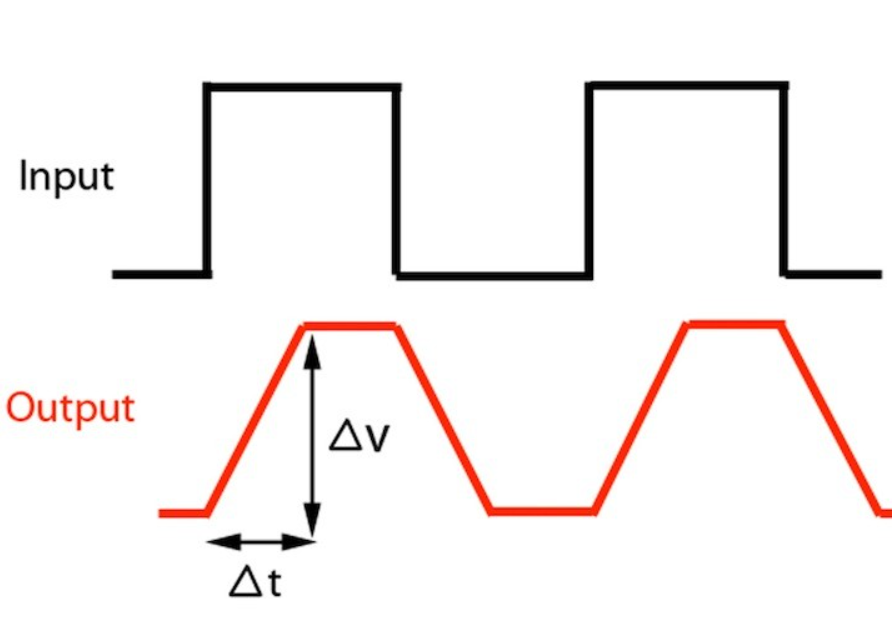
\includegraphics[width=8cm]{Imagenes/sr2.png}
                  \caption{Señal de entrada (negro) y señal de salida (Rojo) esta ultima con un tiempo de retardo por el S.R de la variación de frecuencia.}
                  \label{fig:sr2}
                \end{figure}
                \begin{figure}[H]
                  \centering
                  \renewcommand{\figurename}{Imagen}
                  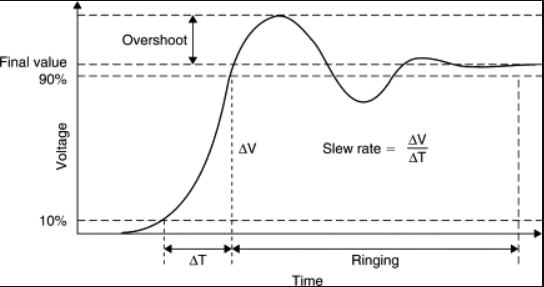
\includegraphics[width=10cm]{Imagenes/sr.png}
                  \caption{Señal de salida y como observar las medidas en el osciloscopio.}
                  \label{fig:sr}
                \end{figure}
    
            \item Limites máximo de excursión

                Se sube solo el voltaje para observar la señal de salida cuando esta se distorsione, recordar que se debe colocar nuevamente la frecuencia en 1KHz

            \item Corriente de corto circuito
                \begin{figure}[H]
                  \centering
                  \setcounter{figure}{25}
                  \includestandalone{Circuitos/bufferv}
                  \caption{Medición de corriente de corto circuito}
                  \label{fig:bufferv}
                \end{figure}

                Para la corriente de cortocircuito, se puede usar la técnica de "\textbf{Resistencia de Carga virtual}",esto es colocar una resistencia virtual en serie con la carga real del circuito, lo que permite medir la caída de tensión a través de la carga virtual.

                La resistencia debe ser lo mas pequeña posible entre $1\si{\ohm}$ y $10\si{\ohm}$, mido la tensión sobre esta resistencia  y por ley de Ohm se puede hallar la corriente de cortocircuito.
        \end{itemize}  
\end{enumerate}

\newpage
\subsection{Parte 3. Filtros Activos}
    \subsubsection{Diseño}
    Para cada uno de los filtros que se muestran en la figura \ref{fig:var_estado}, \ref{fig:sallen_key} y \ref{fig:retro_multiples}.

    \begin{enumerate}
        \item Obtener su modelo circuital de entrada a cada una de sus salidas, observe la importancia de la función de transferencia.

             \begin{figure}[H]
                  \centering
                  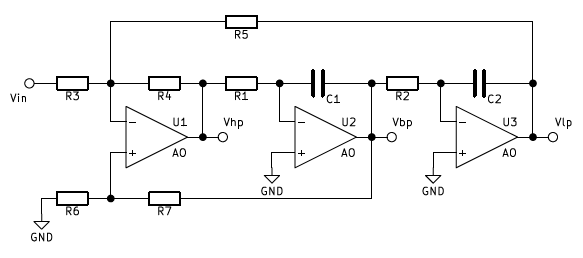
\includegraphics[width=12cm]{Imagenes/var_estado.png}
                  \caption{Filtro de Variables de Estado}
                  \label{fig:var_estado}
            \end{figure}

            Se aplica superposición se halla la salida de cada una de las topologías del circuito de la figura \ref{fig:var_estado}.

            \begin{itemize}
                \item Salida $V_{hp}$
                    \begin{gather}
                        V_{hp}= -\dfrac{R_4}{R_3}V_{in} + \dfrac{R_6}{R_6+R_7}\left(1+\dfrac{R_4}{R_3||R_5}\right)V_{bp}-\dfrac{R_4}{R_5}V_{lp}
                        \label{eqn:vhp}
                    \end{gather}

                \item Salida $V_{bp}$
                    \begin{gather}
                        V_{bp}=-\dfrac{\dfrac{1}{SC_1}}{R_1}V_{hp}=-\dfrac{1}{SC_1R_1}V_{hp}
                        \label{eqn:vbp}
                    \end{gather}

                \item Salida $V_{lp}$
                    \begin{gather}
                        V_{lp}=-\dfrac{\dfrac{1}{SC_2}}{R_2}V_{bp}=-\dfrac{1}{SC_2R_2}V_{bp}
                        \label{eqn:vlp}
                    \end{gather}
            \end{itemize}

            Se hallará la función de transferencia de un filtro pasa bajo, haciendo uso del siguiente sistema de ecuación.
            \begin{equation*}
                \begin{cases}
                    V_{hp}= -\dfrac{R_4}{R_3}V_{in} + \dfrac{R_6}{R_6+R_7}\left(1+\dfrac{R_4}{R_3||R_5}\right)V_{bp}-\dfrac{R_4}{R_5}V_{lp}\\[0.5cm]
                    V_{bp}=-\dfrac{1}{SC_1R_1}V_{hp}\\[0.5cm]
                    V_{lp}=-\dfrac{1}{SC_2R_2}V_{bp}
                \end{cases}
            \end{equation*}

            De la ecuación \ref{eqn:vbp} se despeja $V_{hp}$ y se sustituye en la ecuación \ref{eqn:vhp}, en la ecuación \ref{eqn:vlp} despejamos $V_{bp}$ y se sustituye en \ref{eqn:vhp}, de esta manera se halla $\dfrac{V_{lp}}{V_{in}}$.

            \begin{gather*}
                \begin{cases}
                    V_{bp}=-SC_2R_2V_{lp}\\[0.5cm]
                    V_{hp}=-SC_1R_1V_{bp}
                \end{cases}
            \end{gather*}

            Se sustituye la ecuación $V_{bp}$ en $V_{hp}$.

            \begin{gather*}
                \begin{cases}
                    V_{bp}=-SC_2R_2V_{lp}\\[0.5cm]
                    V_{hp}=-SC_1R_1(-SC_2R_2V_{lp})=S^2C_1C_2R_1R_2V_{lp} 
                \end{cases}
            \end{gather*}

            Se sustituye la ecuación $V_{bp}$ y $V_{hp}$ en la ecuación \ref{eqn:vhp}.
            
            \begin{gather}
                S^2C_1C_2R_1R_2V_{lp}=-\dfrac{R_4}{R_3}V_{in}+ \dfrac{R_6}{R_6+R_7}\left(1+\dfrac{R_4}{R_3||R_5}\right)(-SC_2R_2V_{lp})-\dfrac{R_4}{R_5}V_{lp} \nonumber\\[0.5cm]
                \left[S^2C_1C_2R_1R_2V_{lp}+ \dfrac{R_6}{R_6+R_7}\left(1+\dfrac{R_4}{R_3||R_5}\right)(SC_2R_2V_{lp})+\dfrac{R_4}{R_5}V_{lp}=-\dfrac{R_4}{R_3}V_{in}\right]\dfrac{1}{C_1C_2R_1R_2}\nonumber\\[0.5cm]
                V_{lp}\left[S^2+\dfrac{\dfrac{SR_6}{R_6+R_7}\left(1+\dfrac{R_4}{R_3||R_5}\right)}{C_1R_1}+\dfrac{R_4}{R_5}\dfrac{1}{C_1C_2R_1R_2}\right]=-\dfrac{R_4}{R_3}V_{in}\dfrac{1}{C_1C_2R_1R_2}\nonumber\\[0.5cm]
                \dfrac{V{lp}}{V_{in}}=\dfrac{-\dfrac{R_4}{R_3}\dfrac{1}{C_1C_2R_1R_2}}{S^2+\dfrac{\dfrac{SR_6}{R_6+R_7}\left(1+\dfrac{R_4}{R_3||R_5}\right)}{C_1R_1}+\dfrac{R_4}{R_5}*\dfrac{1}{C_1C_2R_1R_2}} \label{eqn:4}
            \end{gather}
\newpage
            \begin{figure}[H]
                  \centering
                  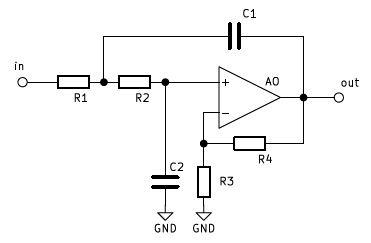
\includegraphics[width=8cm]{Imagenes/sallen_key.png}
                  \caption{Filtro Pasa Bajos con Topologías Sallen-Key}
                  \label{fig:sallen_key}
            \end{figure}

            Se aplica el Método del Amplificador Desvanecido (MAD), aparte se facilitaran los cálculos tomando cada resistencia y capacitancia como admitancias.

            Se le aplicará MAD al Amplificador que tiene configuración no inversora, recordando su formula:

            \begin{gather*}
                A_f=X_{i0}+\dfrac{X_{i1}AX_{30}}{1-X_{31}A}\\[0.5cm]
                A=1+\dfrac{R_4}{R_3}\\[0.5cm]
                X_{i0}=\dfrac{V_0}{V_i}\bigg|_{A=0}=\dfrac{V_iA}{V_i}=0\\[0.5cm]
                X_{i1}=\dfrac{e_1}{V_i}\bigg|_{A=0}=\dfrac{y_1}{y_1+y_2+\dfrac{y_3y_4}{y_3+y_4}}\dfrac{y_3}{y_3+y_4}\\[0.5cm]
                X_{30}=\dfrac{V_0}{e_3}\bigg|_{V_i=0}=\dfrac{V_0}{V_0}=1\\[0.5cm]
                X_{31}=\dfrac{e_1}{e_3}\bigg|_{V_i=0}=\dfrac{y_2}{y_1+y_2+\dfrac{y_3y_4}{y_3+y_4}}\dfrac{y_3}{y_3+y_4}\\[0.5cm]
            \end{gather*}

            Se sustituye cada uno de los valores hallados en la fórmula de MAD, por lo tanto se obtiene lo siguiente:

            \begin{gather}
                A_f=0+\dfrac{\dfrac{y_1}{y_1+y_2+\dfrac{y_3y_4}{y_3+y_4}}\dfrac{y_3}{y_3+y_4}A(1)}{1-A\dfrac{y_2}{y_1+y_2+\dfrac{y_3y_4}{y_3+y_4}}\dfrac{y_3}{y_3+y_4}}=\dfrac{\dfrac{y_1}{\dfrac{(y_1+y_2)(y_3+y_4)+y_3y_4}{y_3+y_4}}\dfrac{y_3}{y_3+y_4}A}{1-A\dfrac{y_2}{\dfrac{(y_1+y_2)(y_3+y_4)+y_3y_4}{y_3+y_4}}\dfrac{y_3}{y_3+y_4}} \nonumber\\[0.5cm]
                A_f=\dfrac{\dfrac{y_1y_3A}{(y_1+y_2)(y_3+y_4)+y_3y_4}}{\dfrac{(y_1+y_2)(y_3+y_4)+y_3y_4-Ay_2y_3}{(y_1+y_2)(y_3+y_4)+y_3y_4}}=\dfrac{y_1y_3A}{(y_1+y_2)(y_3+y_4)+y_3y_4-Ay_2y_3}\nonumber\\[0.5cm]
                A_f=\dfrac{y_1y_3A}{(y_1+y_2+y_4-Ay_2)y_3+y_4(y_1+y_2)}=\dfrac{y_1y_3A}{(y_1+(1-A)y_2+y_4)y_3+y_4(y_1+y_2)}\nonumber\\[0.5cm]
                y_1=\dfrac{1}{R_1}; \quad y_2=SC_1; \quad y_3= \dfrac{1}{R_2}; \quad y_4=SC_2 \nonumber
            \end{gather}

            Se sustituyen cada uno de los valores de $y_1$, $y_2$, $y_3$ y $y_4$, en la ecuación de $A_f$, quedando lo siguiente:

            \begin{gather}
                A_f=\dfrac{\dfrac{1}{R_1}\dfrac{1}{R_2}A}{\left(\dfrac{1}{R_1}+(1+A)SC_1+SC_2\right)\dfrac{1}{R_2}+\left(\dfrac{1}{R_1}+SC_1\right)SC_2}\nonumber\\[0.5cm]
                A_f=\dfrac{\dfrac{A}{R_1R_2}}{\dfrac{1}{R_1R_2}+\dfrac{(1-A)SC_1}{R_2}+\dfrac{SC_2}{R_2}+\dfrac{SC_2}{R_1}+S^2C_1C_2}\nonumber\\[0.5cm]
                A_f=\dfrac{\dfrac{A}{R_1R_2C_1C_2}}{S^2+S\left(\dfrac{(1-A)}{C_2R_2}+\dfrac{1}{C_1R_2}+\dfrac{1}{C_1R_1}\right)+\dfrac{1}{R_1R_2C_1C_2}}\label{eqn:5}
            \end{gather}

\newpage
            \begin{figure}[H]
                  \centering
                  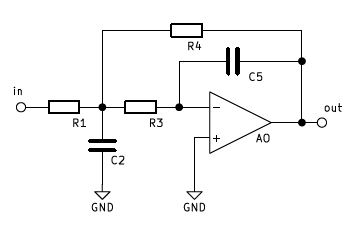
\includegraphics[width=8cm]{Imagenes/retro_multiples.png}
                  \caption{Filtro Pasa Bajos con Topologías de Retroalimentaciones Múltiples}
                  \label{fig:retro_multiples}
            \end{figure}

            Se aplica MAD y para simplificar los cálculos se trabajara en admitancias, al igual que la topología anterior.

            \begin{gather*}
                A=-\dfrac{1}{SC_5R_3}\\[0.5cm] 
                X_{i0}=0; \quad X_{i1}=\dfrac{y_1}{y_1+y_2+y_3+y_4}; \quad X_{30}=1; \quad X_{31}=\dfrac{y_4}{y_1+y_2+y_3+y_4}\\[0.5cm]
                A_f=\dfrac{\dfrac{y_1}{y_1+y_2+y_3+y_4}\left(-\dfrac{1}{SC_5R_3}\right)}{1-\dfrac{y_4}{y_1+y_2+y_3+y_4}\left(-\dfrac{1}{SC_5R_3}\right)}\\[0.5cm]
                A_f=-\dfrac{y_1}{(y_1+y_2+y_3+y_4)(SC_5R_3)+y_4}\\[0.5cm]
                y_1=\dfrac{1}{R_1}; \quad y_2=SC_2; \quad y_3=\dfrac{1}{R_3}; \quad y_4=\dfrac{1}{R_4}
            \end{gather*}

            Se sustituyen cada uno de los valores de $y_1$, $y_2$, $y_3$ y $y_4$, en la ecuación de $A_f$, quedando lo siguiente:

            \begin{gather}
                A_f=\dfrac{-\dfrac{1}{R_1}}{\left(\dfrac{1}{R_1}+SC_2+\dfrac{1}{R_3}+\dfrac{1}{R_4}\right)(SC_5R_3)+\dfrac{1}{R_4}}\nonumber\\[0.5cm]
                A_f=\dfrac{-\dfrac{1}{R_1}}{S^2C_5C_2R_3+SC_5R_3\left(\dfrac{1}{R_1}+\dfrac{1}{R_3}+\dfrac{1}{R_4}\right)+\dfrac{1}{R_4}}\nonumber\\[0.5cm]
                A_f=\dfrac{-\dfrac{1}{R_1R_3C_2C_5}}{S^2+\dfrac{S}{C_2}\left(\dfrac{1}{R_1}+\dfrac{1}{R_3}+\dfrac{1}{R_4}\right)+\dfrac{1}{R_4R_3C_2C_5}} \label{eqn:6}
            \end{gather}

            Recordando que la formula General de filtro pasa bajos es el siguiente:

            \begin{gather}
                H(S)=\dfrac{H_0W_0^2}{S^2+2\zeta w_0S+w_o^2} \label{eqn:HS}
            \end{gather}

        \item Especifique los componentes necesarios, en cada filtro, para obtener frecuencias de corte ($f_0$) de $2.7 KHz$ con factor de amortiguamiento ($\zeta$) de $0.707$, con ganancia de $2$ en la salida pasa bajos.

            \begin{itemize}
                \item \textbf{Filtro de Variables de Estado}
            
            
                    Se hace uso de la ecuación \ref{eqn:HS}, para hallar lo que se pide, empezando con la función de transferencia del filtro de Variables de Estado de la figura \ref{fig:var_estado}, observando la ecuación \ref{eqn:4}, se tiene:
        
                    \begin{gather*}
                        f_0=2.7 KHz ; \quad \zeta=0.707 ; \quad A=2 \\[0.5cm]
                        w_0=2\pi f_o=2\pi (2.7 K)=16.965 K\dfrac{rad}{s}
                    \end{gather*}
        
                    Debido que tenemos tres valores designados como lo son $f_o$, $\zeta$ y $w_0$ y 6 constantes, la cual se deben hallar sus valores para el diseño que se pide, se asumirán distintas constantes permitiendo facilitar el calculo del siguiente sistema de ecuaciones.
        
                    \begin{gather*}
                        \begin{cases}
                            w_0^2=\dfrac{R_4}{R_5C_1C_2R_1R_2}\\[0.5cm]
                            2\zeta w_0=\dfrac{ \dfrac{R_6}{R_6+R_7}\left(1+\dfrac{R_4}{R_3||R_5}\right)}{C_1R_1}\\[0.5cm]
                            H_0w_0^2=-\dfrac{R_4}{R_3}\dfrac{1}{C_1C_2R_1R_2}
                        \end{cases}
                    \end{gather*}
        
                    Se sustituye $w_0^2$ en $H_0w_0^2$ y de esta última despejamos $H_0$.
        
                    \begin{gather*}
                        H_0=-\dfrac{1}{w_0^2}\dfrac{R_4}{R_3}\dfrac{1}{C_1C_2R_1R_2}=-\dfrac{1}{\dfrac{R_4}{R_5C_1C_2R_1R_2}}\dfrac{R_4}{R_3}\dfrac{1}{C_1C_2R_1R_2}\\[0.5cm]
                        H_0=-\dfrac{R_5}{R_3}=-2 \quad \therefore \quad R_5=2R_3
                    \end{gather*}
        
                    Se asume que $R_5=10.2 K \ohm \quad \therefore \quad R_3=5.1K\ohm$ 
                    
                    Asumiendo valores a $C_1=C_2=10nF$ y tomando $R_5$ en la ecuación $w_0^2$, se tiene:
        
                    \begin{gather*}
                        w_0^2=\dfrac{R_4}{C_1C_2R_1R_2R_5}\\[0.5cm]
                        C_1C_2w_0^2=\dfrac{R_4}{R_1R_2R_5}
                    \end{gather*}
        
                    Asumiendo $R_1=3.3k\ohm$ y $R_2=2.2K\ohm$
        
                    \begin{gather*}
                        R_4=C_1C_2w_0^2R_1R_2R_5\\[0.5cm]
                        R_4=(10n)^2(16.965K)^2(3.3K)(2.2K)(10.2K)=2131.3 \approx 2.2K\ohm
                    \end{gather*}
        
                    Ahora se hace uso de los valores anteriormente hallados, para encontrar $R_6$ y $R_7$ en la ecuación $2\zeta w_0$ 
        
                    \begin{gather*}
                        2\zeta w_0=\dfrac{\dfrac{R_6}{R_6+R_7}\left(1+\dfrac{R_4}{R_3||R_5}\right)}{C_1R_1}\\[0.5cm]
                        R_3||R_5=\dfrac{R_3R_5}{R_3+R_5}= \dfrac{5.1K(10.2K)}{5.1K+10.2K}=3.4k\ohm\\[0.5cm]
                        2(0.707)(16.965K)=\dfrac{1}{10n(3.3K}\dfrac{R_6}{R_6R_7}\left(1+\dfrac{2.2K}{3.4K}\right)\\[0.5cm]
                        0.79162= \dfrac{R_6}{R_6R_7}(1.64705)\\[0.5cm]
                        \dfrac{0.79162}{1.64705}= \dfrac{R_6}{R_6R_7} \Longrightarrow 0.4806(R_6+R_7)=R_6 \Longrightarrow 0.4806R_7=0.51937R_6\\[0.5cm]
                        R_7=1.08R_6 \approx R_6
                    \end{gather*}
        
                    Teniendo en cuenta que $R_7\approx R_6$ se asume, $$R_7=R_6=10K\ohm$$
        
                    Asimismo se realizará para los filtros de la figura \ref{fig:sallen_key} y \ref{fig:retro_multiples}, continuamos con la Topología Sallen-Key.

                \item \textbf{Filtro Pasa Bajos con Topología Sallen-Key}
                
                    Como se indica en el proceso anterior, se hará uso de la ecuación \ref{eqn:HS} y la función de transferencia del filtro pasa bajos de la topología de Sallen-Key que es la ecuación \ref{eqn:5}. Obteniendo el siguiente sistema de ecuaciones:
        
                    \begin{gather*}
                        \begin{cases}
                            w_0^2=\dfrac{1}{R_1R_2C_1C_2}\\[0.5cm]
                            2\zeta w_0=\dfrac{(1-A)}{C_2R_2}+\dfrac{1}{C_1R_2}+\dfrac{1}{C_1R_1}=\dfrac{R_4}{C_2R_3R_2}+\dfrac{1}{C_1R_2}+\dfrac{1}{C_1R_1}\\[0.5cm]
                            H_0w_0^2=\dfrac{1}{R_1R_2C_1C_2}\dfrac{R_3+R_4}{R_3}
                        \end{cases}
                    \end{gather*}
        
                    Se sustituye $w_0^2$ en $H_0w_0^2$, obteniendo lo siguiente:
        
                    \begin{gather*}
                        H_0=\dfrac{1}{w_0^2}\dfrac{1}{R_1R_2C_1C_2}\dfrac{R_3+R_4}{R_3}\\[0.5cm]
                        H_0=\dfrac{1}{\dfrac{1}{R_1R_2C_1C_2}}\dfrac{1}{R_1R_2C_1C_2}\dfrac{R_3+R_4}{R_3}\\[0.5cm]
                        H_0=\dfrac{R_3+R_4}{R_3}=2 \Longrightarrow 2R_3=R_3+R_4 \Longrightarrow 2R_3-R_3=R_4\\[0.5cm]
                        R_3=R_4
                    \end{gather*}
        
                    Por esa razón, se asume que $$R_3=R_4=1K\ohm$$
        
                    Con los datos hallados los sustituimos en $2\zeta w_0$, de esa manera se halla $R_1$ y $R_2$. Se asume que $C_1=C_2=\SI{10}{\nano\farad}$

                    \begin{gather*}
                        2\zeta w_0= \dfrac{R_4}{C_2R_3R_2}+\dfrac{1}{C_1R_2}+\dfrac{1}{C_1R_1}\\[0.5cm]
                        2\zeta w_0=\dfrac{1}{R_2}\left(\dfrac{R_4}{C_1R_4}+\dfrac{1}{C_1}\right)+\dfrac{1}{C_1R_1}=\dfrac{2}{R_2C_1}+\dfrac{1}{C_1R_1}\\[0.5cm]
                        2\zeta w_0=\dfrac{2C_1R_1+R_2C_1}{C_1^2R_2R_1}=\dfrac{2R_1+R_2}{C_1R_2R_1}
                    \end{gather*}

                    Se asume que $R_1=3.9K\ohm$ y $R_2=8.2K\ohm$

                \item \textbf{Filtro Pasa Bajos con topología de retroalimentaciones múltiples}

                    Se toma en cuenta nuevamente la ecuación \ref{eqn:HS} y \ref{eqn:6}. Se forma el siguiente sistema de ecuaciones:

                    \begin{gather*}
                        \begin{cases}
                            w_0^2=\dfrac{1}{R_4R_3C_2C_5}\\[0.5cm]
                            H_0w_0^2=-\dfrac{1}{R_1R_3C_2C_5}\\[0.5cm]
                            2\zeta w_0=\dfrac{1}{C_2}\left(\dfrac{1}{R_1}+\dfrac{1}{R_3}+\dfrac{1}{R_4}\right)
                        \end{cases}
                    \end{gather*}

                    Se sustituye la ecuación $w_0^2$ en $H_0w_0^2$, se obtiene:

                    \begin{gather*}
                        H_0=-\dfrac{1}{w_0^2}\dfrac{1}{R_1R_3C_2C_5}=-\dfrac{1}{\dfrac{1}{R_4R_3C_2C_5}}\dfrac{1}{R_1R_3C_2C_5}=-\dfrac{R_4}{R_1}\\[0.5cm]
                        H_0=-2=-\dfrac{R_4}{R_1} \Longrightarrow R_4=2R_1
                    \end{gather*}

                    Por consiguiente, se asume que $R_1=1K\ohm '\quad \therefore \quad R_4=2K \approx 2.2k\ohm$

                    Ahora se usará la ecuación $2\zeta w_0$, para hallar $R_3$, asumiendo que $C_2=80nF$ y $C_5=10nF$

                    \begin{gather*}
                        2\zeta w_0=\dfrac{1}{C_2}\left(\dfrac{1}{R_1}+\dfrac{1}{R_3}+\dfrac{1}{R_4}\right)=\dfrac{1}{C_2}\left(\dfrac{2}{R_4}+\dfrac{1}{R_3}+\dfrac{1}{R_4}\right)\\[0.5cm]
                        2\zeta w_0C_2=\dfrac{3}{R_4}+\dfrac{1}{R_3}\\[0.5cm]
                        2(0.707)(2 \pi 2.7K)(80n)-\dfrac{3}{2.2K}=\dfrac{1}{R_3}=555.4\mu\\[0.5cm]
                        R_3=\dfrac{1}{555.4\mu}=1.8K\ohm
                    \end{gather*}

                    Se busca que $R_3$ y $R_4$ sean iguales, por lo tanto, $$R_3=R_4=1.8K\approx 2.2K$$
            \end{itemize}
        \subsubsection{Simulación}
        \item Verifique sus diseños, mediante simulación, comparando la Respuesta en frecuencia obtenida, con el diagrama asintótico de Bode de cada filtro. Determine la ganancia de cada filtro a las frecuencias en las que planea medir la Respuesta en frecuencia.

        \begin{itemize}
            \item \textbf{Filtro de Variables de Estado}

                Se muestra la siguiente tabla que indica los valores de las resistencias usadas en cada simulación, previamente calculadas tras su diseño.

                \begin{table}[H]
                    \centering
                    \begin{tabular}{|c|c|}
                        \hline
                        \textbf{Componente} & \textbf{Valor} \\\hline
                        $\mathbf{R_1}$ &  $3.3k\si{\ohm}$ \\\hline
                        $\mathbf{R_2}$ & $2.2k \si{\ohm}$  \\\hline
                        $\mathbf{R_3}$ & $3.1k \si{\ohm}$  \\\hline
                        $\mathbf{R_4}$ & $2.2k \si{\ohm}$   \\\hline
                        $\mathbf{R_5}$ & $10k\si{\ohm}$  \\\hline
                        $\mathbf{R_6}$  & $10k\si{\ohm}$ \\\hline
                        $\mathbf{R_7}$  & $10k\si{\ohm}$ \\\hline
                        $\mathbf{C_1}$  & $\SI{10}{\nano\farad}$ \\\hline
                        $\mathbf{C_2}$  & $\SI{10}{\nano\farad}$ \\\hline
                    \end{tabular}
                    \caption{Valores de los componentes que diseña un filtro pasa bajo de variables de estado}
                    \label{tab:diseño_var_estado}
                \end{table}

                \begin{figure}[H]
                      \centering
                      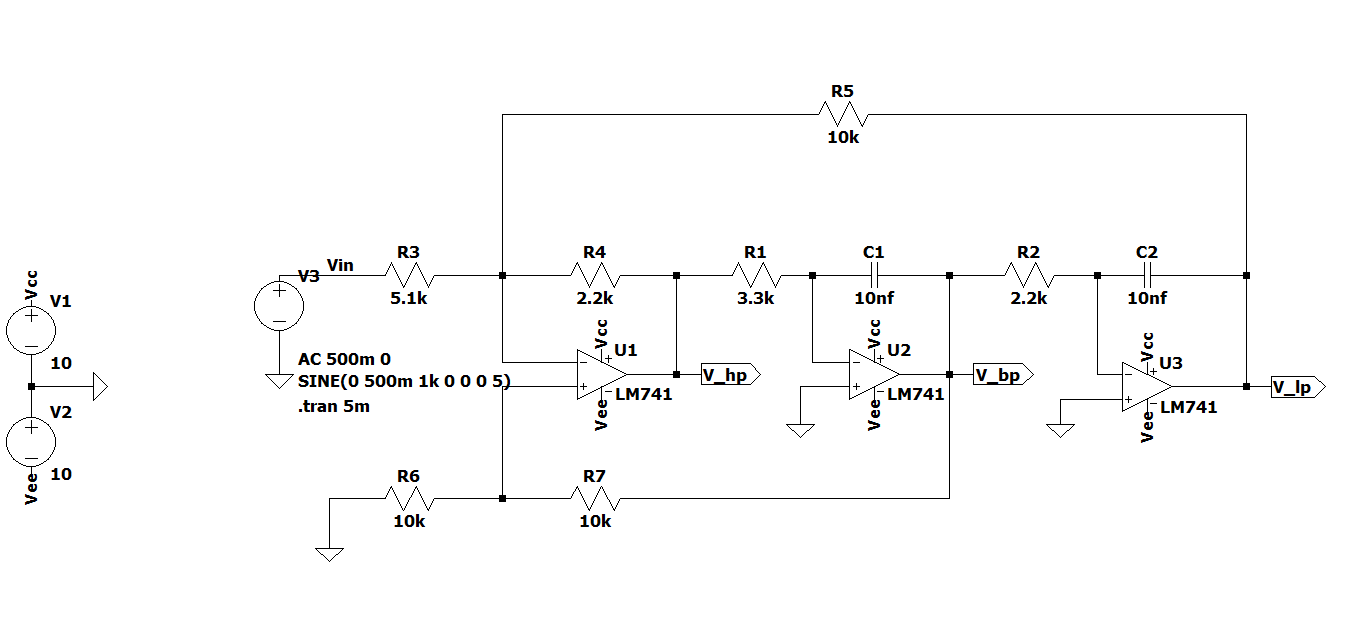
\includegraphics[width=15cm]{Imagenes/sim_var_estado_circuito.png}
                      \caption{Diseño del Filtro de Variables de Estado pasa bajos}
                      \label{fig:sim_var_estado_circuito}
                \end{figure}

                \begin{figure}[H]
                      \centering
                      \renewcommand{\figurename}{Gráfica}
                      \setcounter{figure}{8}
                      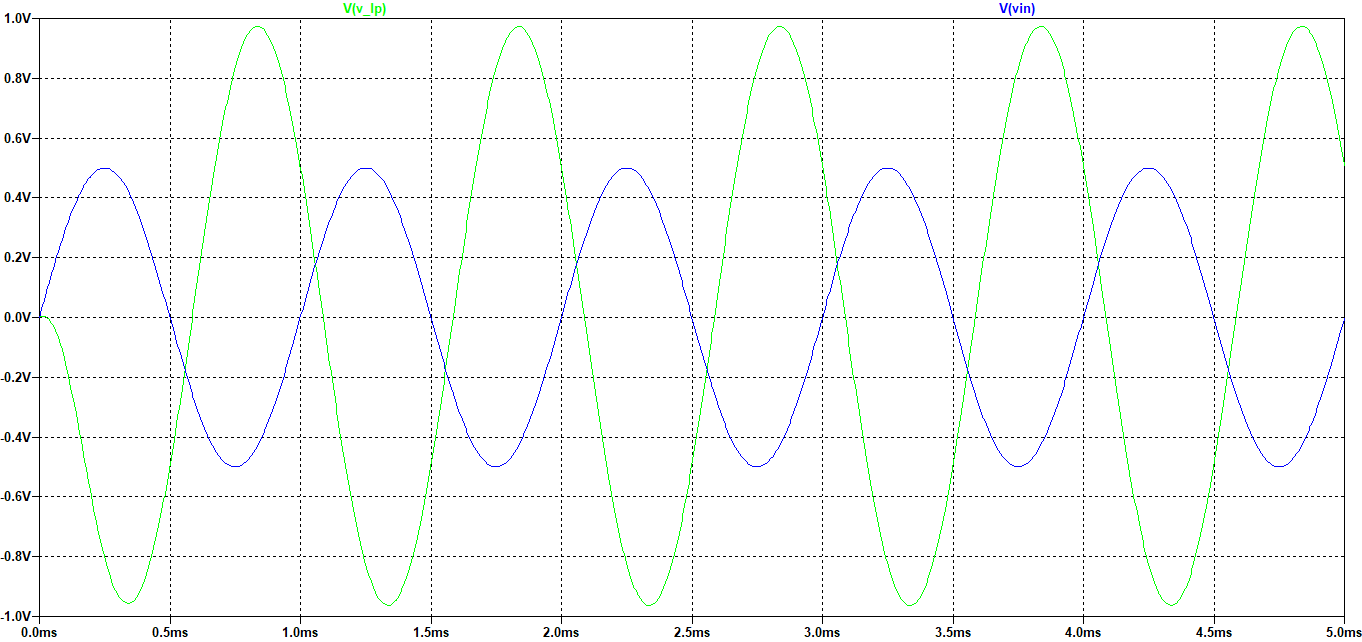
\includegraphics[width=15cm]{Imagenes/sim_var_estado_vo.png}
                      \caption{Señal de Salida y Entrada del Diseño del Filtro de Variables de Estado pasa bajos}
                      \label{fig:sim_var_estado_vo}
                \end{figure}

                Como se puede observar en la gráfica \ref{fig:sim_var_estado_vo} se obtiene una ganancia de -2, como la que se realizo en el diseño. Por consiguiente, falta añadir el diagrama de Bode para verificar si fue un  diseño adecuado a la respuesta en frecuencia deseada.

                \begin{figure}[H]
                      \centering
                      \renewcommand{\figurename}{Gráfica}
                      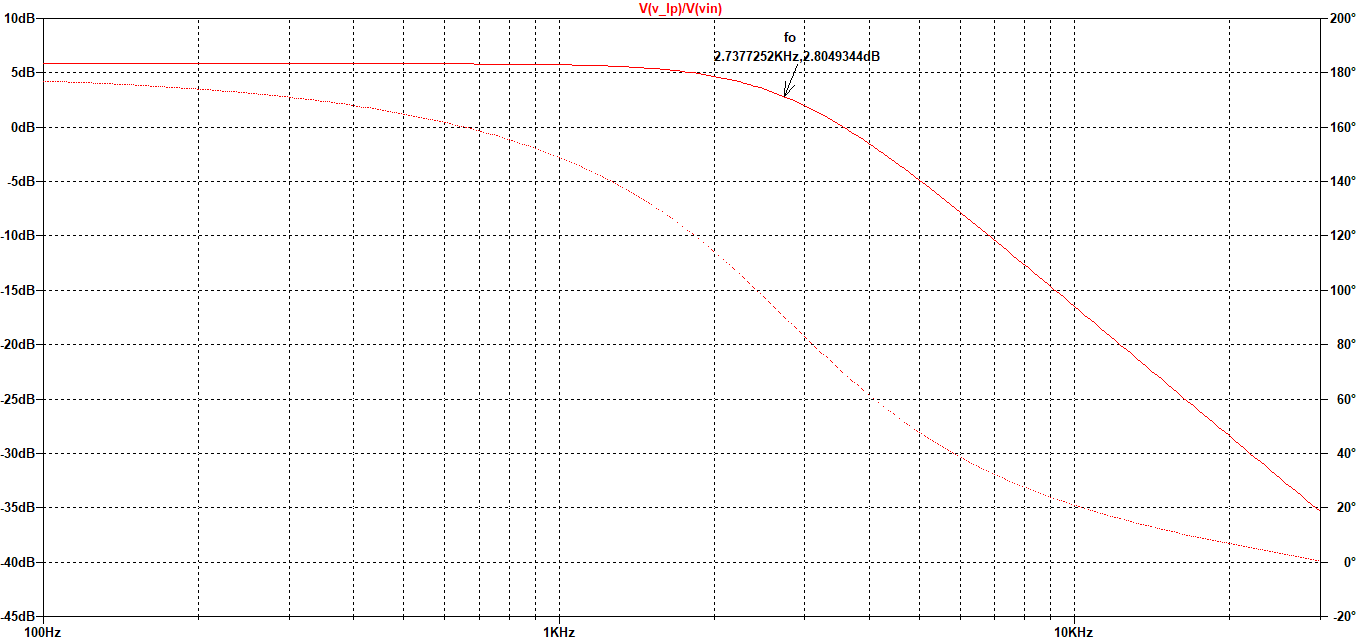
\includegraphics[width=15cm]{Imagenes/sim_var_estado_bode.png}
                      \caption{Diagrama de Bode (Magnitud y Fase) del Diseño del Filtro de Variables de Estado pasa bajos. Frecuencia de corte señalada en negro}
                      \label{fig:sim_var_estado_bode}
                \end{figure}

                Efectivamente los cálculos realizados en el diseño del  filtro son los correctos, para las condiciones deseadas en el laboratorio.

            \item \textbf{Filtro Pasa Bajos con Topología Sallen-Key}

                \begin{table}[H]
                    \centering
                    \begin{tabular}{|c|c|}
                        \hline
                        \textbf{Componente} & \textbf{Valor} \\\hline
                        $\mathbf{R_1}$ &  $3.9k\si{\ohm}$ \\\hline
                        $\mathbf{R_2}$ & $8.2k \si{\ohm}$  \\\hline
                        $\mathbf{R_3}$ & $1k \si{\ohm}$  \\\hline
                        $\mathbf{R_4}$ & $1k \si{\ohm}$   \\\hline
                        $\mathbf{C_1}$  & $\SI{10}{\nano\farad}$ \\\hline
                        $\mathbf{C_2}$  & $\SI{10}{\nano\farad}$ \\\hline
                    \end{tabular}
                    \caption{Valores de los componentes que diseña un filtro pasa bajo con topología Sallen-Key}
                    \label{tab:diseño_sallen_key}
                \end{table}

                \begin{figure}[H]
                      \centering
                      \setcounter{figure}{30}
                      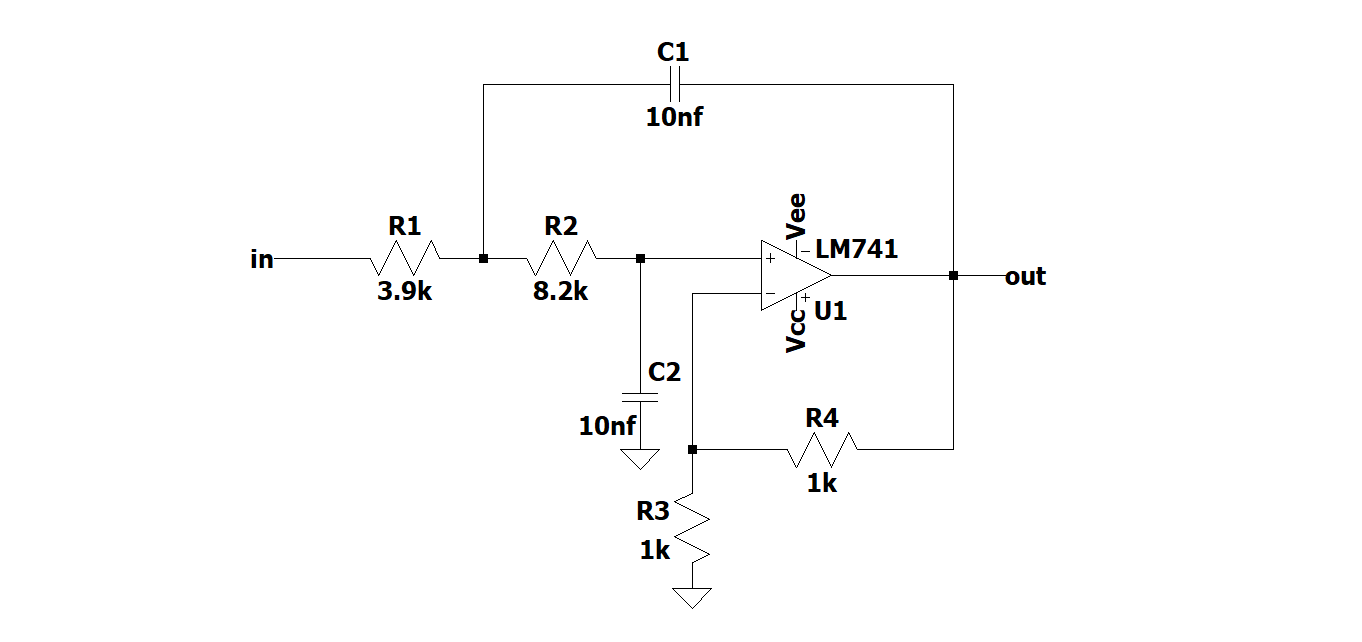
\includegraphics[width=15cm]{Imagenes/sim_sallen_key_circuito.png}
                      \caption{Diseño del Filtro pasa bajos con topología Sallen-Key}
                      \label{fig:sim_sallen_key_circuito}
                \end{figure}

                \begin{figure}[H]
                      \centering
                      \renewcommand{\figurename}{Gráfica}
                      \setcounter{figure}{10}
                      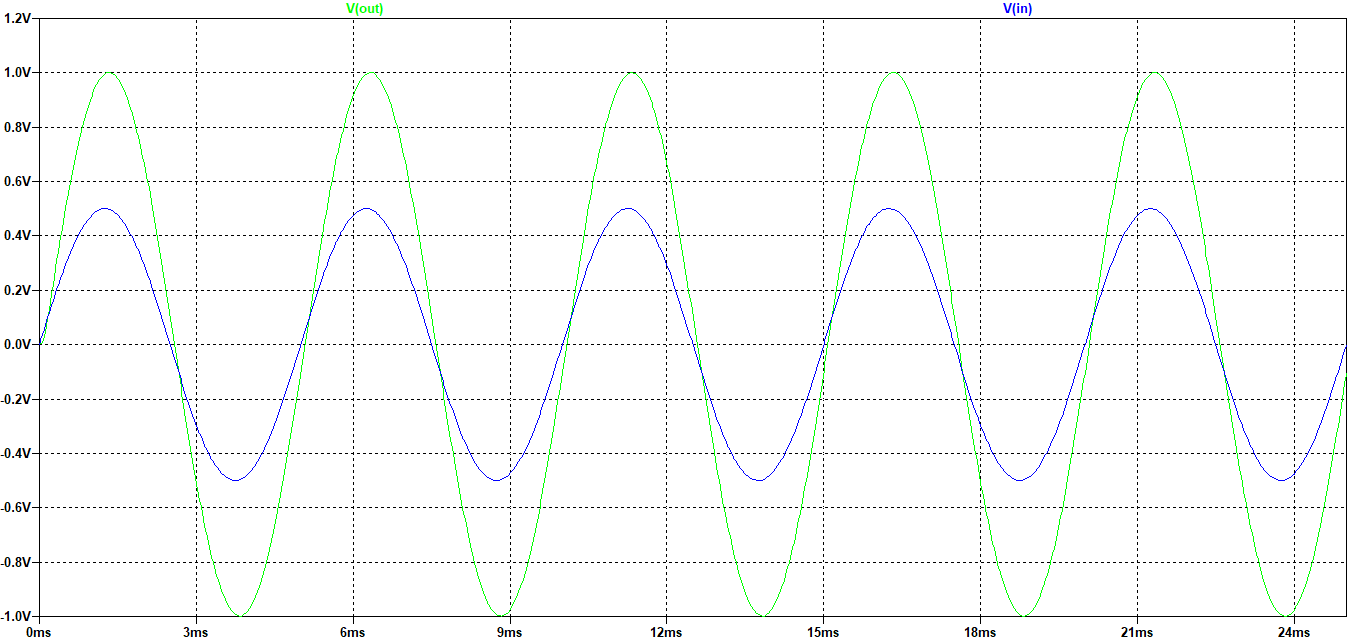
\includegraphics[width=15cm]{Imagenes/sim_sallen_key_vo.png}
                      \caption{Señal de Salida y Entrada del Diseño del Filtro pasa bajos con topología Sallen-Key}
                      \label{fig:sim_sallen_key_vo}
                \end{figure}

                \begin{figure}[H]
                      \centering
                      \renewcommand{\figurename}{Gráfica}
                      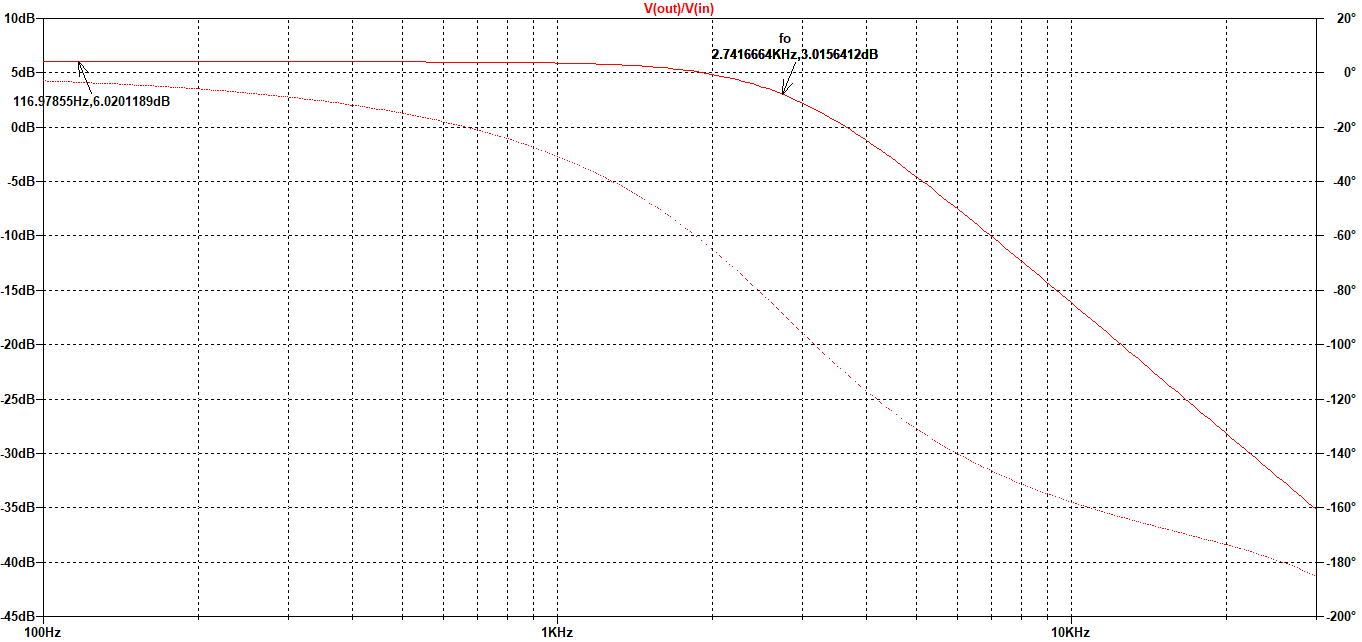
\includegraphics[width=15cm]{Imagenes/sim_sallen_key_bode.png}
                      \caption{Diagrama de Bode (Magnitud y Fase) del Diseño del Filtro pasa bajos con topología Sallen-Key. Frecuencia de corte señalada en negro}
                      \label{fig:sim_sallen_key_bode}
                \end{figure}

                Como se visualiza en las gráficas   \ref{fig:sim_sallen_key_vo} y \ref{fig:sim_sallen_key_bode}, Se obtuvo una ganancia de 2, una frecuencia de corte de 2.7 KHz, con su error relativo apreciable, sin embargo, no deja de ser preciso.

            \item \textbf{Filtro Pasa Bajos con topología de retroalimentaciones múltiples}   

                \begin{table}[H]
                    \centering
                    \begin{tabular}{|c|c|}
                        \hline
                        \textbf{Componente} & \textbf{Valor} \\\hline
                        $\mathbf{R_1}$ &  $1k\si{\ohm}$ \\\hline
                        $\mathbf{R_3}$ & $2.2k \si{\ohm}$  \\\hline
                        $\mathbf{R_4}$ & $2.2k \si{\ohm}$   \\\hline
                        $\mathbf{C_2}$  & $\SI{80}{\nano\farad}$ \\\hline
                        $\mathbf{C_5}$  & $\SI{10}{\nano\farad}$ \\\hline
                    \end{tabular}
                    \caption{Valores de los componentes que diseña un filtro pasa bajo con topología de retroalimentaciones múltiples}
                    \label{tab:diseño_retro}
                \end{table}

                \begin{figure}[H]
                      \centering
                      \setcounter{figure}{31}
                      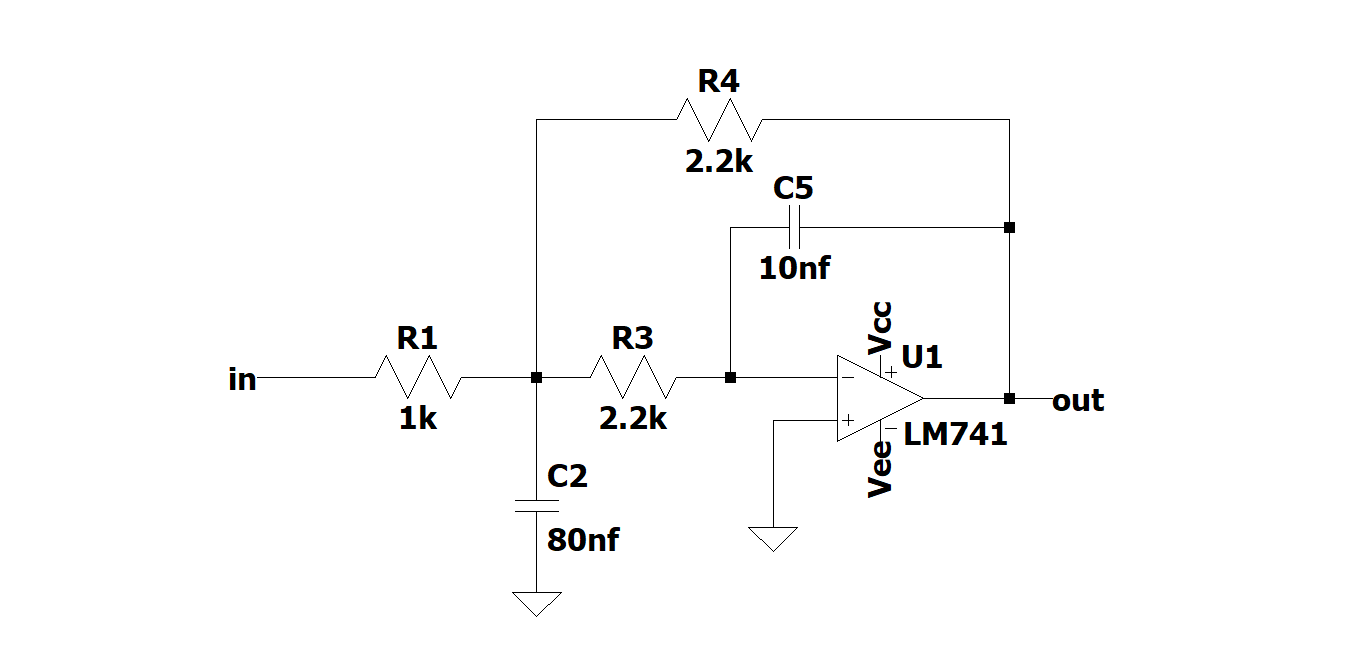
\includegraphics[width=15cm]{Imagenes/sim_retro_circuito.png}
                      \caption{Diseño del Filtro pasa bajos con topología de retroalimentaciones múltiples}
                      \label{fig:sim_retro_circuito}
                \end{figure}

                \begin{figure}[H]
                      \centering
                      \renewcommand{\figurename}{Gráfica}
                      \setcounter{figure}{12}
                      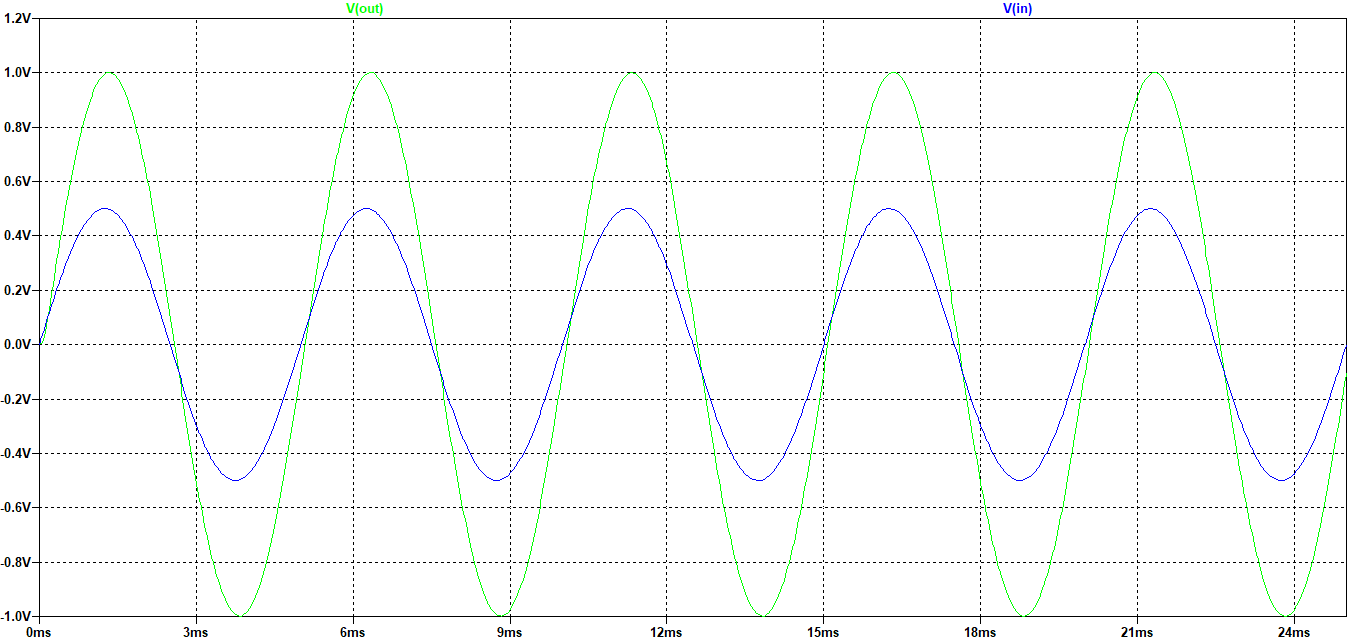
\includegraphics[width=15cm]{Imagenes/sim_sallen_key_vo.png}
                      \caption{Señal de Salida y Entrada del Diseño del Filtro pasa bajos con topología de retroalimentaciones múltiples}
                      \label{fig:sim_retro_vo}
                \end{figure}

                \begin{figure}[H]
                      \centering
                      \renewcommand{\figurename}{Gráfica}
                      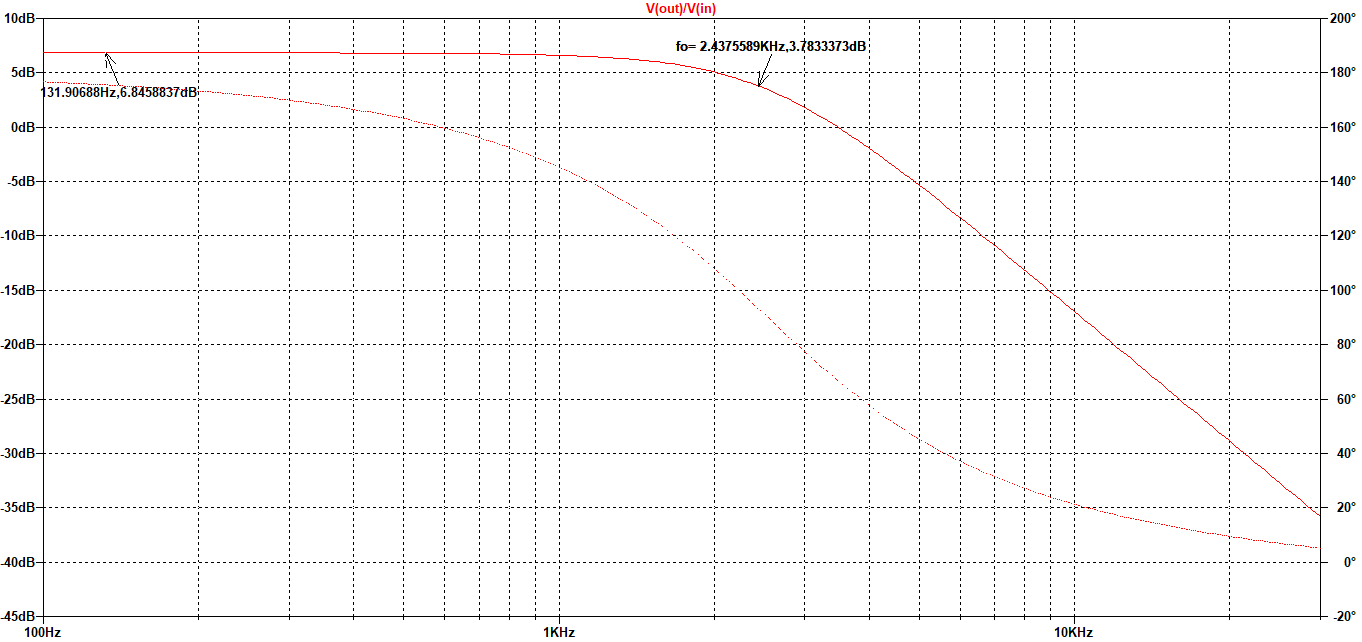
\includegraphics[width=15cm]{Imagenes/sim_retro_bode.png}
                      \caption{Diagrama de Bode (Magnitud y Fase) del Diseño del Filtro pasa bajos con topología de retroalimentaciones múltiples. Frecuencia de corte señalada en negro}
                      \label{fig:sim_retro_bode}
                \end{figure}

                Acá si se obtiene una salida distinta como se ve en la gráfica \ref{fig:sim_retro_vo}, donde su salida es un poco mayor que 2, sin embargo, entra dentro de lo tolerable, también se observa una frecuencia de corte menor. Por consiguiente, se logrará realizar en el laboratorio cada una de las topologías que se diseño, para saber si se ajusta a las condiciones que se desean, reflejando los cálculos teóricos y las simulaciones en  la práctica.                
        \end{itemize}

        \item Por simulación obtenga las formas en cada salida al inyectar señales cuadradas con frecuencia tal, que su tercera armónica, coincida con la frecuencia de corte indicadas. Explique a que se deben las formas de onda obtenidas.

            Para hallar esa frecuencia que se le dará a la onda cuadrada, en especifico que se su tecera armonica, coincida con la frecuencia de corte indicada anteriormente, se debe realizar lo siguiente:

            \begin{gather*}
                T=\dfrac{1}{f_o} r\\[0.5cm]
                \text{Lo que se hará a continuación es hallar la frecuencia fundamental, asumiendo que la} \\[0.5cm]
                \text{frecuencia de corte es su tercer armónico, logrando la condición necesaria}\\[0.5cm]
                f_1=\dfrac{f_o}{3}=\dfrac{2.7KHz}{3}=900Hz\\[0.5cm]
                \text{siendo esta la frecuencia fundamental que se le colocará a la onda cuadrada}\\[0.5cm]
                T_1=\dfrac{1}{f_1}=\dfrac{1}{900}=1.111ms
            \end{gather*}

            Debido a las simulaciones anteriores, ya se sabe que cada frecuencia de corte dependiendo de su topología, y el diseño que se realizo, poseen pequeñas variaciones, sin embargo se ajustará de igual manera a 900 Hz y se observará su frecuencia de corte.

            Las ondas resultantes son consecuencia de las variaciones inducidas por la señal de entrada, que en este caso es una onda cuadrada. Al emplear esta forma de onda como entrada, se generan armónicos debido a la presencia de cambios abruptos en la señal. Además, en cada topología de filtro, se incorporan capacitores como elementos del circuito. Estos capacitores introducen más armónicos debido a sus propiedades con la corriente alterna, contribuyendo así a la complejidad de la respuesta de frecuencia del sistema.

            Es crucial destacar que la presencia de armónicos puede afectar el rendimiento del circuito. Sin embargo, la implementación de filtros activos, como los estudiados en este apartado, juega un papel crucial en mitigar los efectos negativos de estos armónicos. Al diseñar estos filtros específicos, se logra atenuar selectivamente ciertos componentes armónicos, preservando así la integridad y estabilidad del circuito frente a las variaciones no deseadas generadas por la onda cuadrada de entrada.

            \begin{itemize}
                \item \textbf{Filtro de Variables de Estado}

                    \begin{figure}[H]
                          \centering
                          \renewcommand{\figurename}{Gráfica}
                          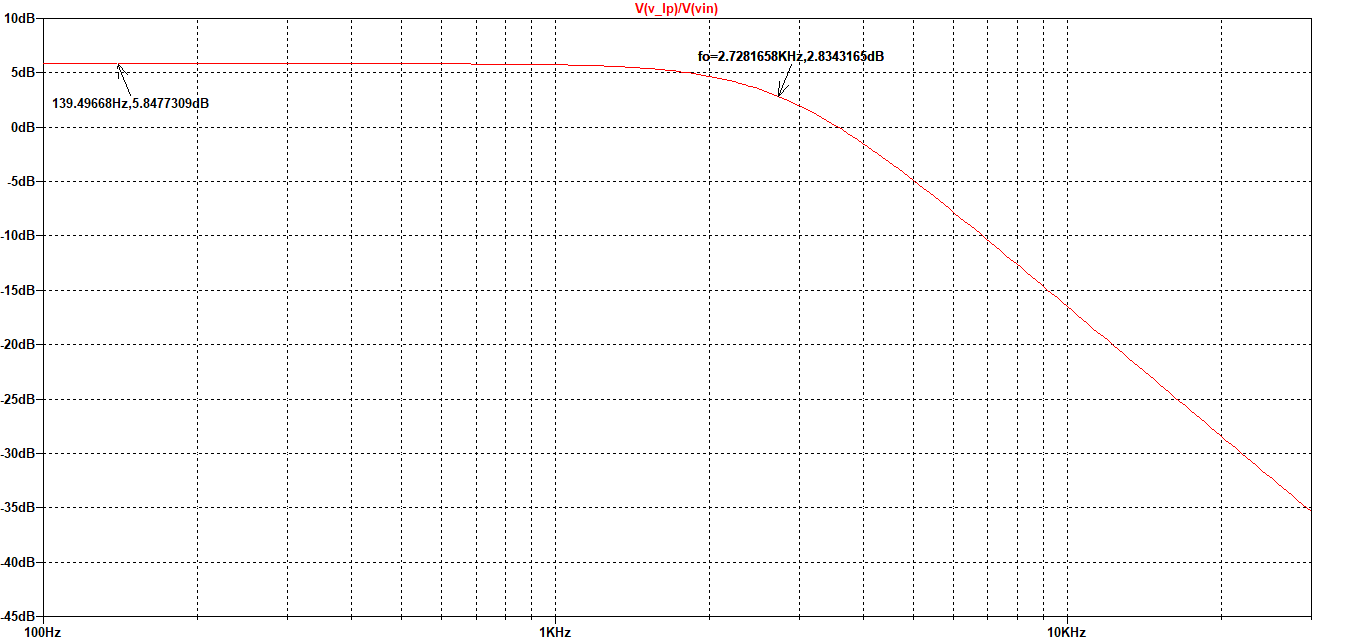
\includegraphics[width=15cm]{Imagenes/sim_var_estado_armonico_bode.png}
                          \caption{Diagrama de Bode de Magnitud del Diseño del Filtro de variables de estados pasa bajos. Frecuencia de corte señalada en negro}
                          \label{fig:sim_var_estado_armonico_bode}
                    \end{figure}

                    \begin{figure}[H]
                      \centering
                      \renewcommand{\figurename}{Gráfica}
                      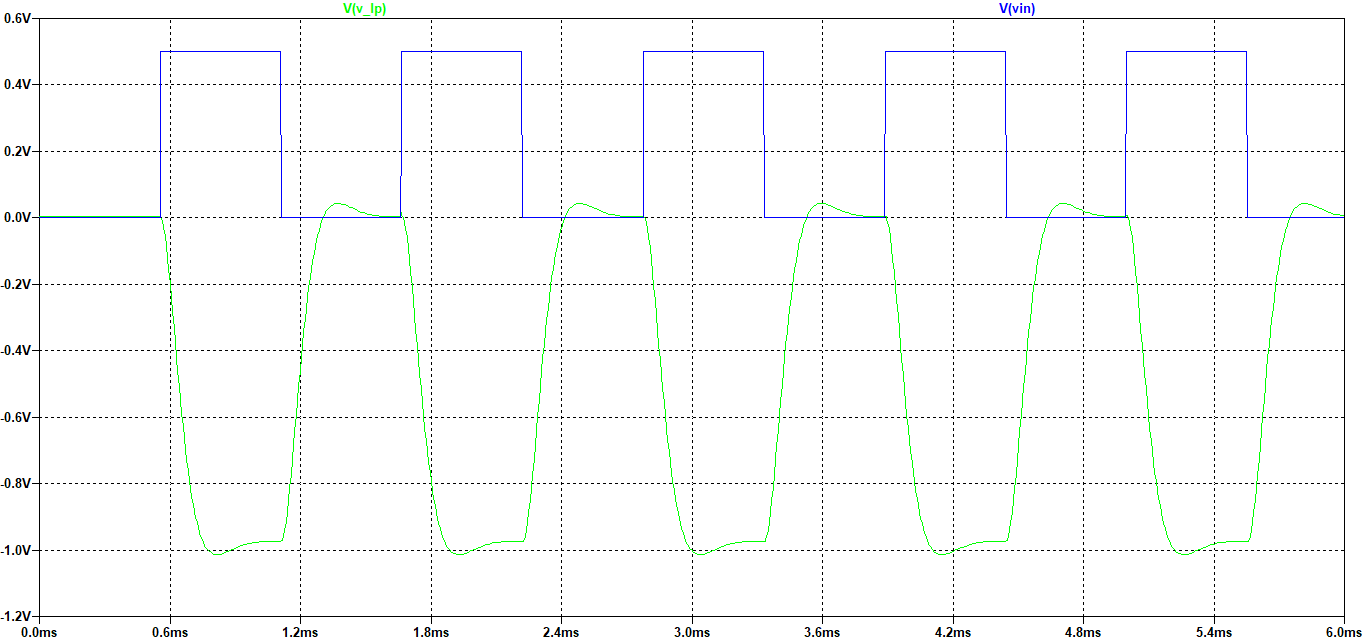
\includegraphics[width=15cm]{Imagenes/sim_var_estado_armonico_vo.png}
                      \caption{Señal de Salida y Entrada del Diseño del Filtro de variables de estados pasa bajos}
                      \label{fig:sim_var_estado_armonico_vo}
                \end{figure}

                
                
                \item \textbf{Filtro Pasa Bajos con Topología Sallen-Key}

                    \begin{figure}[H]
                          \centering
                          \renewcommand{\figurename}{Gráfica}
                          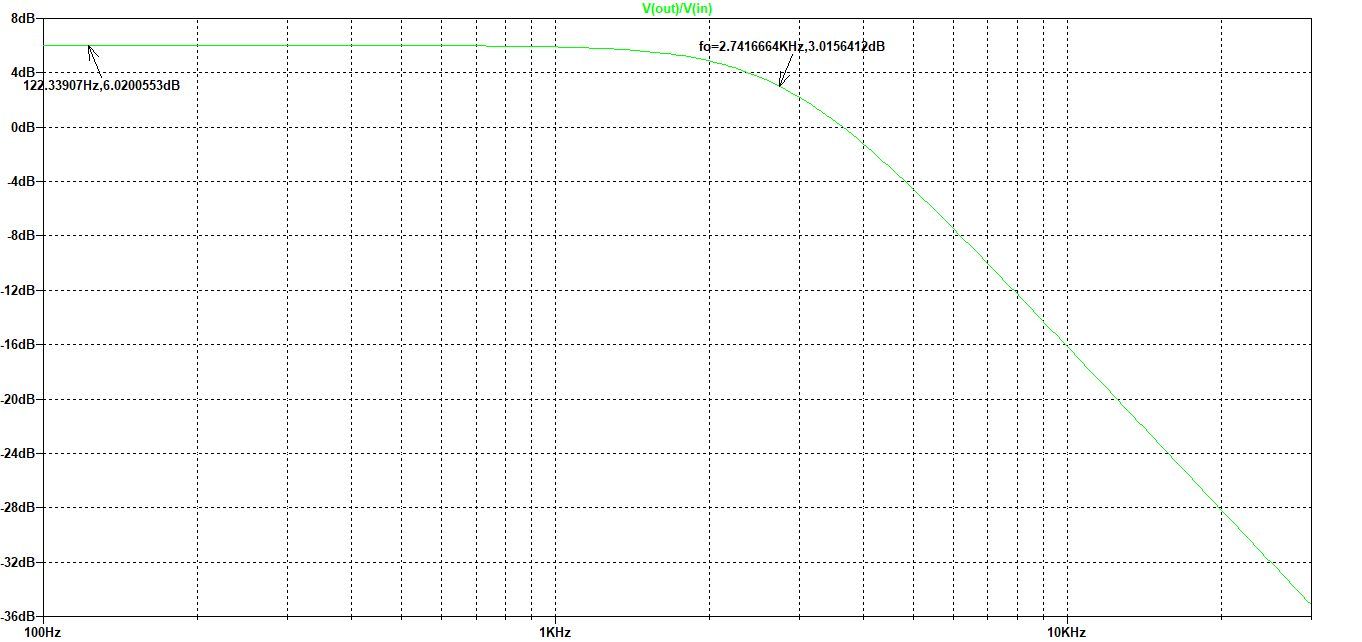
\includegraphics[width=15cm]{Imagenes/sim_sallen_key_armonico_bode.png}
                          \caption{Diagrama de Bode de Magnitud del Diseño del Filtro Pasa Bajos con Topología Sallen-Key. Frecuencia de corte señalada en negro}
                          \label{fig:sim_sallen_key_armonico_bode}
                    \end{figure}

                    \begin{figure}[H]
                      \centering
                      \renewcommand{\figurename}{Gráfica}
                      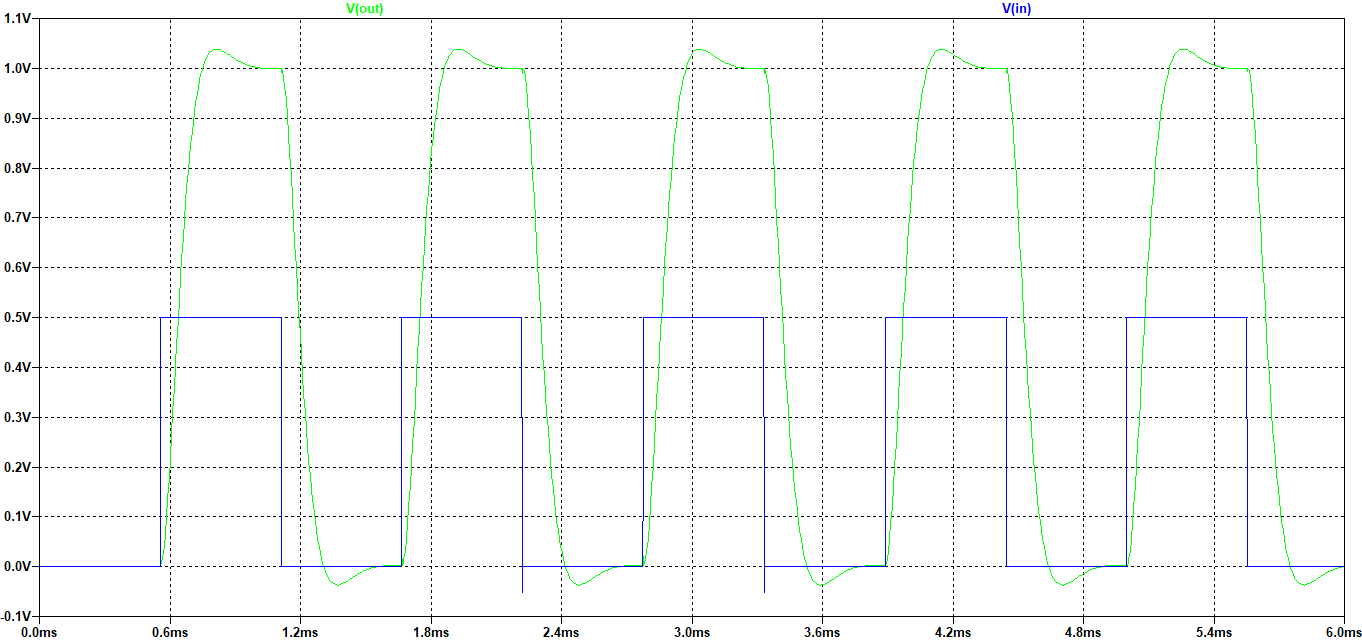
\includegraphics[width=15cm]{Imagenes/sim_sallen_key_armonico_vo.png}
                      \caption{Señal de Salida y Entrada del Diseño del Filtro Pasa Bajos con Topología Sallen-Key}
                      \label{fig:sim_sallen_key_armonico_vo}
                    \end{figure}    
                    
                \item \textbf{Filtro Pasa Bajos con topología de retroalimentaciones múltiples} 

                    \begin{figure}[H]
                          \centering
                          \renewcommand{\figurename}{Gráfica}
                          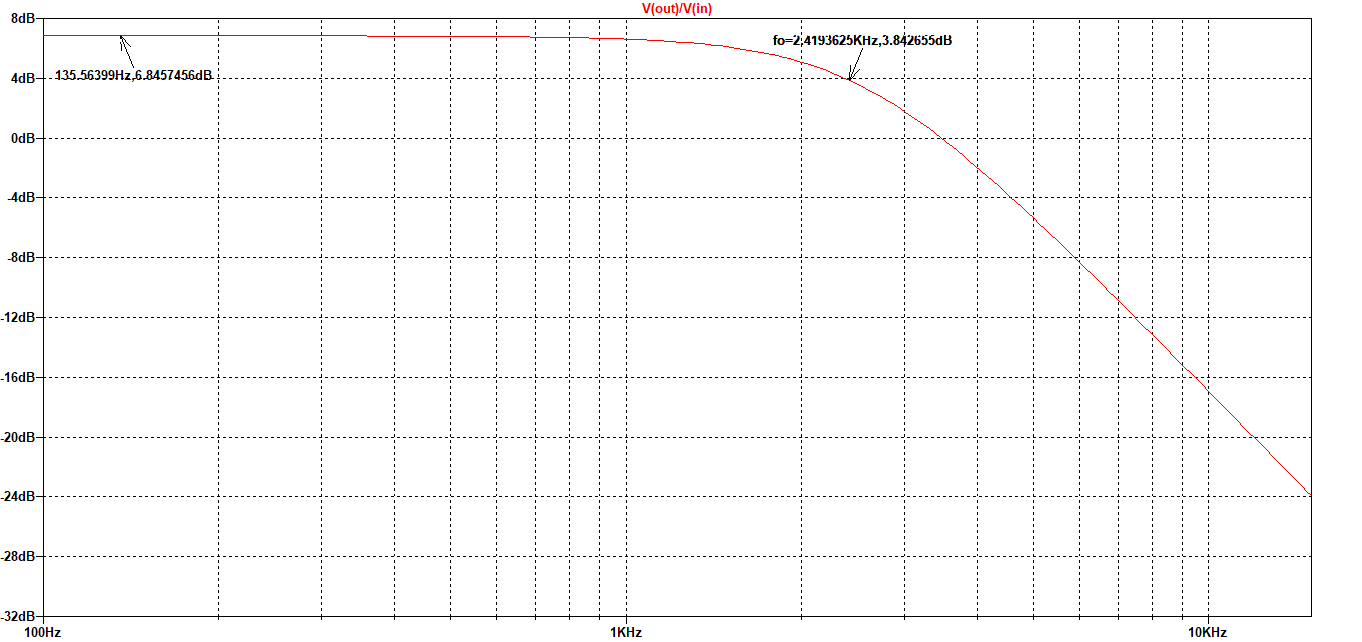
\includegraphics[width=15cm]{Imagenes/sim_retro_armonico_bode.png}
                          \caption{Diagrama de Bode de Magnitud del Diseño del Filtro Pasa Bajos con topología de retroalimentaciones múltiples. Frecuencia de corte señalada en negro}
                          \label{fig:sim_retro_armonico_bode}
                    \end{figure}

                    \begin{figure}[H]
                      \centering
                      \renewcommand{\figurename}{Gráfica}
                      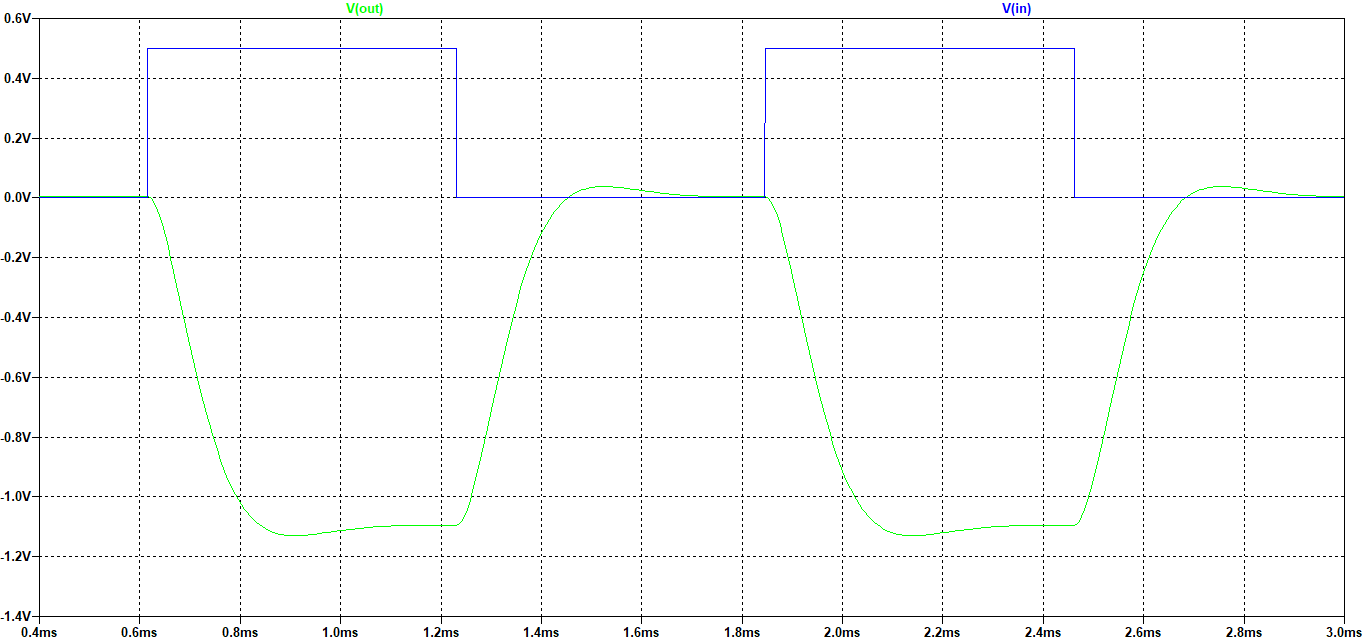
\includegraphics[width=15cm]{Imagenes/sim_retro_armonico_vo.png}
                      \caption{Señal de Salida y Entrada del Diseño del Filtro Pasa Bajos con topología de retroalimentaciones múltiples}
                      \label{fig:sim_retro_armonico_vo}
                    \end{figure}
            \end{itemize}

            Al observar las gráficas \ref{fig:sim_var_estado_armonico_vo}, \ref{fig:sim_sallen_key_armonico_vo} y \ref{fig:sim_retro_armonico_vo} de la señal de salida, se aprecia una curva suave en el tiempo de retardo, resultado de la presencia del tercer armónico. Esta característica contribuye a que la salida se asemeje considerablemente a la forma de onda de entrada. No obstante, es importante destacar que este fenómeno tiene un propósito específico: transformar el circuito en un filtro eficaz.

            La estrategia es limitar la propagación de armónicos no deseados, asegurando que la salida actúe como un filtro a partir del momento en que el tercer armónico alcanza la frecuencia de corte predeterminada. Esta transición se evidencia claramente en las gráficas, donde se puede observar cómo el circuito controla selectivamente los armónicos, permitiendo que solo aquellos hasta el tercer armónico afecten la señal de salida antes de aplicar el filtrado necesario para cumplir con los requisitos del diseño.
    \end{enumerate}

\newpage
\subsection{Parte 4. Fuentes Lineales y Reguladores Monolíticos}
    \subsubsection{Diseño}
    \begin{figure}[H]
          \centering
          \setcounter{figure}{32}
          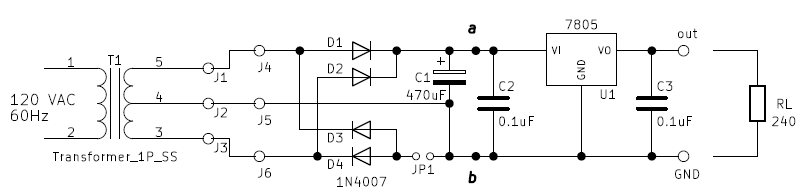
\includegraphics[width=15cm]{Imagenes/regulador_sal_fija.png}
          \caption{Regulador con Tensión de Salida Fija con Center Tap (solo tomando D1 y D2}
          \label{fig:regulador_sal_fija}
    \end{figure}

    \begin{enumerate}
        \item Para la fuente regulada de $5\volt$ fija de la figura \ref{fig:regulador_sal_fija}:
            \begin{enumerate}
                \item Explique la función de los condensadores $C_2$ y $C_3$.

                    Estos capacitores se utilizan para filtrar el ruido y las fluctuaciones en el voltaje de entrada del regulador. Ayuda a estabilizar la tensión debido a $C_1$ que permite que la inda positiva posea un voltaje de rizado, mejorar la respuesta transitoria y reducir la interferencia  electromagnética. Esto último debido a $C_2$, ya que este es el acoplador, permitiendo filtrar corrientes y/o voltajes indebidos.

                \item Explique como conectar el puente de diodos si el transformador no tiene toma central (CT).

                    Se coloca un puente de diodos sin necesidad del center tap.

                    \begin{figure}[H]
                        \centering
                        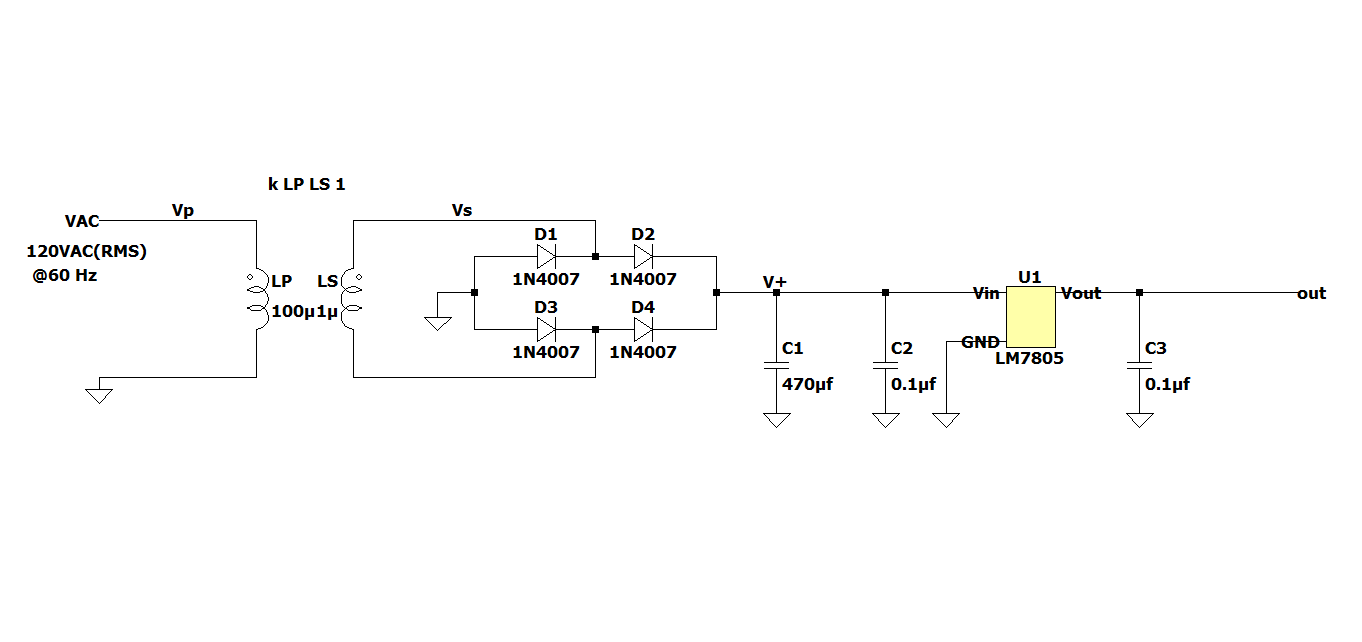
\includegraphics[width=15cm]{Imagenes/reg_sinct.png}
                        \caption{Regulador con Tensión de Salida Fija sin Center Tap}
                        \label{fig:reg_sinct}
                    \end{figure}

                    De esta manera como se observa en la figura \ref{fig:reg_sinct} se obtiene una regulación con tensión de salida fija, permitiendo hacer una rectificación de onda completa.

                \item Suponiendo una carga de 80mA determine la tensión de rizado pico-pico que se va a presentar en $C_1$.

                    Una carga de 80mA, es de $R_L=62.5 \approx 68\ohm$, siendo este último el valor comercial.
                    \begin{gather}
                        V_r= \dfrac{I_{DC}}{2fC}\label{eqn:vr}\\[0.5cm]
                        V_r=\dfrac{80mA}{2(60)(470\mu)}=1.418\volt\nonumber\\[0.5cm]
                        \text{Se halla su $V_{rpp}$}\nonumber\\[0.5cm]
                        V_{rpp}=1.418(\sqrt{2})\approx 2\volt\nonumber
                    \end{gather}

                \item Determine la tensión mínima del secundario del transformador en función de la corriente de salida, de manera que el regulador pueda mantener la regulación. Soporte sus cálculos con datos obtenidos en las hojas de datos del regulador (y marca) que usted va a usar.

                    Como se puede observar en el apartado de los anexos, capitulo \ref{sec:anexos} se tiene el datasheet del regulador 7805, para indicar cual es el valor de entrada requerido para poder obtener 5 voltios de salida. 

                    Indicando que el voltaje de entrada deberían ser los siguientes: $$7\leq V_{in} \leq 25$$

                    Haciendo uso de la ecuación \ref{eqn:vmin} se tiene:

                    \begin{gather}
                        V_{min} = V_s\sqrt{2} - \dfrac{V_{rp}}{2} - 2V_d \label{eqn:vmin}\\[0.5cm]
                        \text{Despejando $V_s$, recordar que el resultado será en RMS}\nonumber \\[0.5cm]
                        V_s = \dfrac{1}{\sqrt{2}}\left(V_{min} + \dfrac{V_{rp}}{2} + 2V_d\right)\label{eqn:vsrms}\\[0.5cm]
                        \text{Si usamos los valores mínimos y máximos de entrada en la ecuación \ref{eqn:vsrms}, se obtiene lo siguiente:}\nonumber \\[0.5cm]
                        V_{min} = 7\volt \nonumber \\[0.5cm]
                        V_s = \dfrac{1}{\sqrt{2}}\left(7 + \dfrac{2}{2} + 2(0.7)\right) = 6.6468\volt \nonumber\\[0.5cm]
                        V_{max} = 25 \volt \nonumber \\[0.5cm]
                        V_s = \dfrac{1}{\sqrt{2}}\left(25 + \dfrac{2}{2} + 2(0.7)\right) = 19.37\volt \nonumber
                    \end{gather}

                \item Determine la relación que va a obtener al colocar unas cargas de 100mA, recuerde que 
                \begin{gather}
                    reg=\dfrac{V_{occ}-V_{osc}}{V_{osc}}100\%
                    \label{eqn:regulacion}
                \end{gather}
                

                    \begin{gather*}
                        V_{osc}=5V\\[0.5cm]
                        V_{occ}=IR=100m(50)=5V \quad\therefore \quad reg=\dfrac{5-5}{5}=0\%
                    \end{gather*}

                    Indicando el resultado con una carga de 50 $\ohm$ que mantiene su voltaje de salida, siendo una regulación efectiva.
            \end{enumerate}

        \item Para la fuente regulada de la figura \ref{fig:regulador_sal_ajustable}

            \begin{figure}[H]
                \centering
                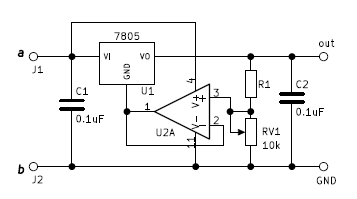
\includegraphics[width=8cm]{Imagenes/regulador_sal_ajustable.png}
                \caption{Regulador con Tensión de Salida Ajustable}
                \label{fig:regulador_sal_ajustable}
            \end{figure}

            \begin{enumerate}
                \item Determinar el rango de tensiones de salida en función del accionamiento <<x>>

                    \begin{gather}
                        I=\dfrac{5\volt}{R_1} \quad ; \quad V_2=I(xR_{v1}) \nonumber\\[0.5cm]
                        \text{Sustituyendo $I$ y $V_2$, en la siguiente ecuación}\nonumber\\[0.5cm]
                        V_o=5\volt+V_2 \Longrightarrow V_o=5\volt+I(xR_{v1})=5V+\dfrac{5\volt}{R_1}(xR_{v1})\nonumber\\[0.5cm]
                        V_o=5\left(1+\dfrac{xR_{v1}}{R_1}\right)\label{1}\\[0.5cm]
                        \text{los valores de  $0\leq x \leq 1$}   \nonumber
                    \end{gather}

                \item Asigne el valor de $R_1$ con el fin de que la fuente suministre tensiones hasta al menos 15V.

                    Tomando en cuenta que el valor de $x=1$, se tiene lo siguiente de la ecuación \ref{1}:

                    \begin{gather}
                        V_o=15\volt=5\volt\left(1+\dfrac{\SI{10}{\kilo\ohm}}{R_1}\right)\Longrightarrow \dfrac{15\volt}{5\volt}=3=1+\dfrac{\SI{10}{\kilo\ohm}}{R_1}\nonumber\\[0.5cm]
                        R_1=\dfrac{10k}{2}=\SI{5}{\kilo\ohm}
                    \end{gather}

                \item Determinar la corriente de polarización que suministra el amplificador operacional 

                    La corriente de polarización es la corriente que pasa por la resistencia $R_1$, por lo tanto,
                    
                    \begin{gather*}
                        I=\dfrac{5\volt}{R_1}= \dfrac{5\volt}{R_1}=1mA
                    \end{gather*}

                \item Determinar la tensión minima de secundario del transformador en función de la corriente de salida, de manera que el regulador puede mantener la regulación.

                    Se usa la ecuación \ref{eqn:vsrms} y sustituyendo $V_r$ por la ecuación \ref{eqn:vr}, se tiene:

                    \begin{gather}
                        V_s = \dfrac{1}{\sqrt{2}}\left(V_{min} + \dfrac{I_{DC}}{4fC} + 2V_d\right) \nonumber\\[0.5cm]
                        V_s = \dfrac{1}{\sqrt{2}}\left(15 + \dfrac{I_{DC}}{4(60)(470\mu)} + 1.4\right) \nonumber\\[0.5cm]
                        V_s = 11.6+6.268 I_{DC} \label{eqn:vsidc}               
                    \end{gather}

                    Ahora con la ecuación \ref{eqn:vsidc}, dándole valores a $I_{DC}$ se obtienen distintos valores del voltaje del secundario del transformador

                    \begin{itemize}
                        \item $I_{DC}=0$

                            $$V_s=11.6\volt$$
                        \item $I_{DC}=1mA$

                            $$V_s=11.6\volt$$
                        \item $I_{DC}=100mA$

                            $$V_s=12.226\volt$$
                    \end{itemize}
            \end{enumerate}

        \item Para la fuente de corriente ajustable de la figura \ref{fig:fuente_corriente_variable}.

            \begin{figure}[H]
                \centering
                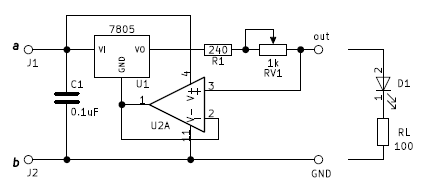
\includegraphics[width=8cm]{Imagenes/fuente_corriente_variable.png}
                \caption{Fuente de corriente variable}
                \label{fig:fuente_corriente_variable}
            \end{figure}
            \begin{enumerate}
                \item Determinar el rango de corrientes de salida en función del accionamiento x.

                    \begin{gather}
                        I_o=\dfrac{V_o}{R_1+xR_{v1}} \label{2}
                    \end{gather}

                    Con la ecuación \ref{2}, se tienen los siguientes casos:

                    \begin{equation}
                        I_o =
                        \begin{cases}
                            20.83 \, \mathrm{mA}, & \quad \text{si } x = 0; \\[0.5cm]
                            \dfrac{5}{240+x(1k)} \, \mathrm{mA}, & \quad \text{si } 0 < x < 1; \\[0.5cm]
                            4.03 \, \mathrm{mA}, & \quad \text{si } x = 1.
                        \end{cases}
                    \end{equation}
            \end{enumerate}

        \item Para cada uno de los montajes anteriores:
            \begin{enumerate}
                \item Determine las potencias en cada elemento que vaya a usar, incluyendo las resistencias de carga.

                    \begin{itemize}
                        \item Figura \ref{fig:regulador_sal_fija}

                        
                            Se sabe que 
                            \begin{gather}
                                P=VI=\dfrac{V^2}{R} \label{p},
                            \end{gather}
                            
                             por lo tanto, se tiene:

                           \begin{gather*}
                                R_{L1} = 240 \, \Omega \quad ; \quad R_{L2} = 60 \, \Omega \\
                                P_{R_{L1}} = \frac{5^2}{240} = 104.16 \, \mathrm{mW} \quad ; \quad P_{R_{L2}} = \frac{5^2}{60} = 36.76 \, \mathrm{mW}
                            \end{gather*}

                        \item Figura \ref{fig:regulador_sal_ajustable}

                            Se usa la ecuación \ref{p}, se tiene,

                            \begin{table}[H]
                                \centering
                                \begin{tabular}{|c|c|}
                                    \hline
                                    \textbf{$P_{R_1}$}                   & \textbf{$x$} \\ \hline
                                    $(1 \, m)^2(5 \, k)=5 \, mW$         & $0$          \\ \hline
                                    $5 \, mW < P < 1.6667 \, mW$         & $0<x<1$      \\ \hline
                                    $\dfrac{5^2}{15 \, k}= 1.6667 \, mW$ & $1$          \\ \hline
                                \end{tabular}
                                \caption{Potencias de los elementos resistivos.}
                            \end{table}

                    \item Figura \ref{fig:fuente_corriente_variable}

                        Se usa la ecuación \ref{p}, se tiene,

                        \begin{table}[h]
                          \centering
                          \begin{tabular}{|c|c|}
                            \hline
                            \textbf{$P_{R_1}$} & \textbf{x} \\
                            \hline
                            $20.83 \, m^2 (240) = 104.13 \, mW$ & 0 \\
                            \hline
                            $20.83 \, m^2 (240 + 1k) = 538.02 \, mW$ & 1 \\
                            \hline
                          \end{tabular}
                          \caption{Potencia de los elementos resistivos}
                        \end{table}
                    \end{itemize}
    \subsubsection{Diseño}
    
                \item Por simulación verifique cada uno de los items anteriores (aquellos que sean susceptibles de hacerlo).
                    \begin{itemize}
                        \item  Se observara la salida de la figura \ref{fig:reg_sinct} con distintas cargas y así determinar si los cálculos realizados son los adecuados para la práctica.
                    
                   


                            \begin{figure}[H]
                                \centering
                                \renewcommand{\figurename}{Gráfica}
                                \setcounter{figure}{20}
                                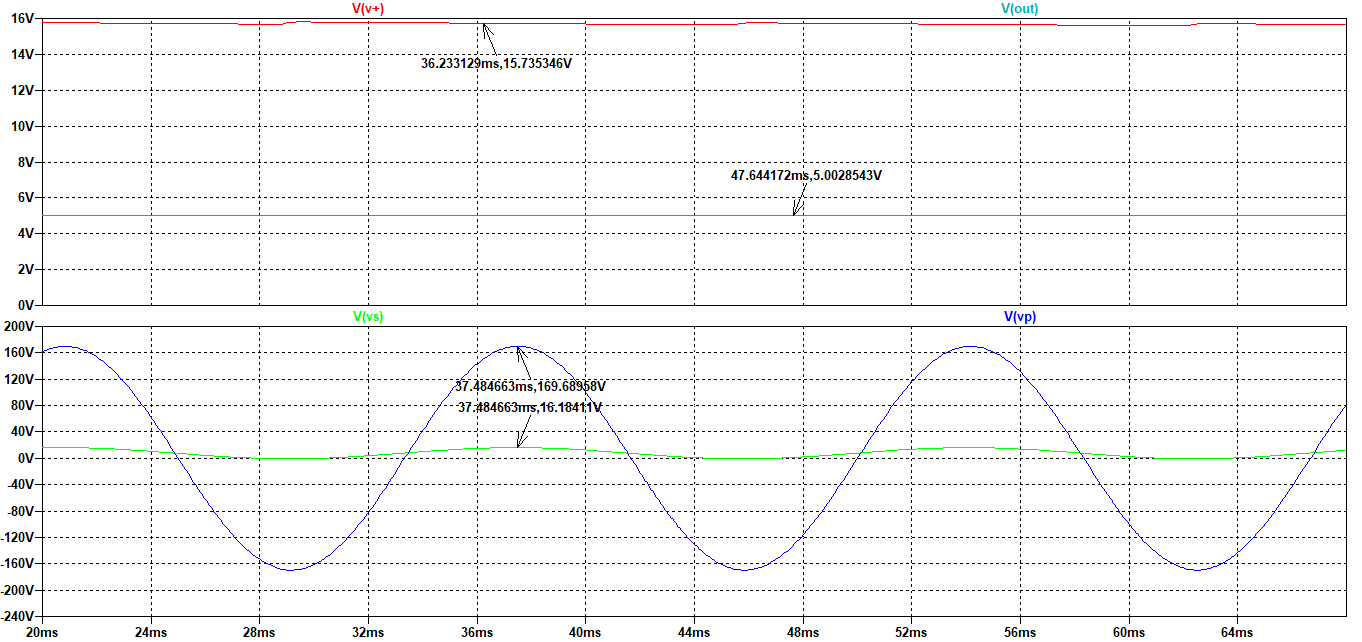
\includegraphics[width=15cm]{Imagenes/sim_reg_sinct.png}
                                \caption{Voltaje de salida del regulador (V(out)), Voltaje del primario (V(vp)), Voltaje del secundario (V(vs)), Voltaje de salida del puente de diodos junto al rizado (V(v+))}
                                \label{fig:sim_reg_sinct}
                            \end{figure}
        
        
                            \begin{figure}[H]
                                \centering
                                \renewcommand{\figurename}{Gráfica}
                                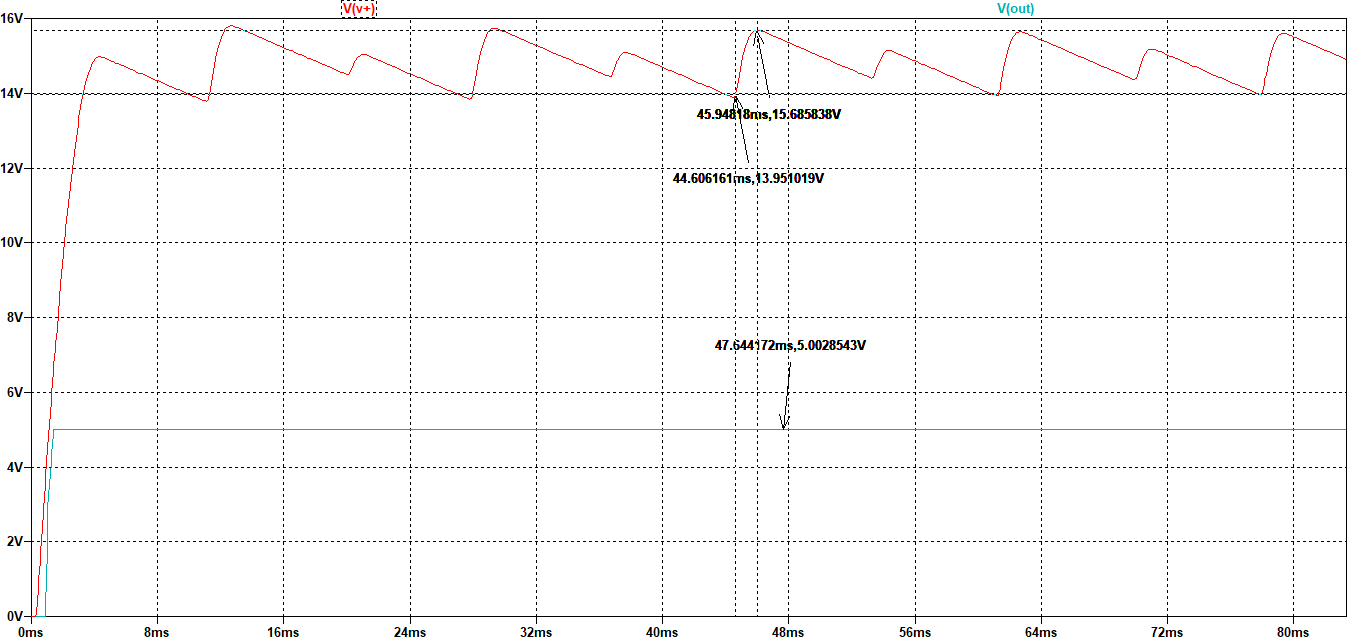
\includegraphics[width=15cm]{Imagenes/sim_reg_sinct_rl.png}
                                \caption{Voltaje de salida del regulador (V(out)), Voltaje de salida del puente de diodos junto al rizado (V(v+)) con una carga de 68 ohms, dando un voltaje de rizado de 1.73 V}
                                \label{fig:sim_reg_sinct_rl}
                            \end{figure}
        
        
                            \begin{figure}[H]
                                \centering
                                \renewcommand{\figurename}{Gráfica}
                                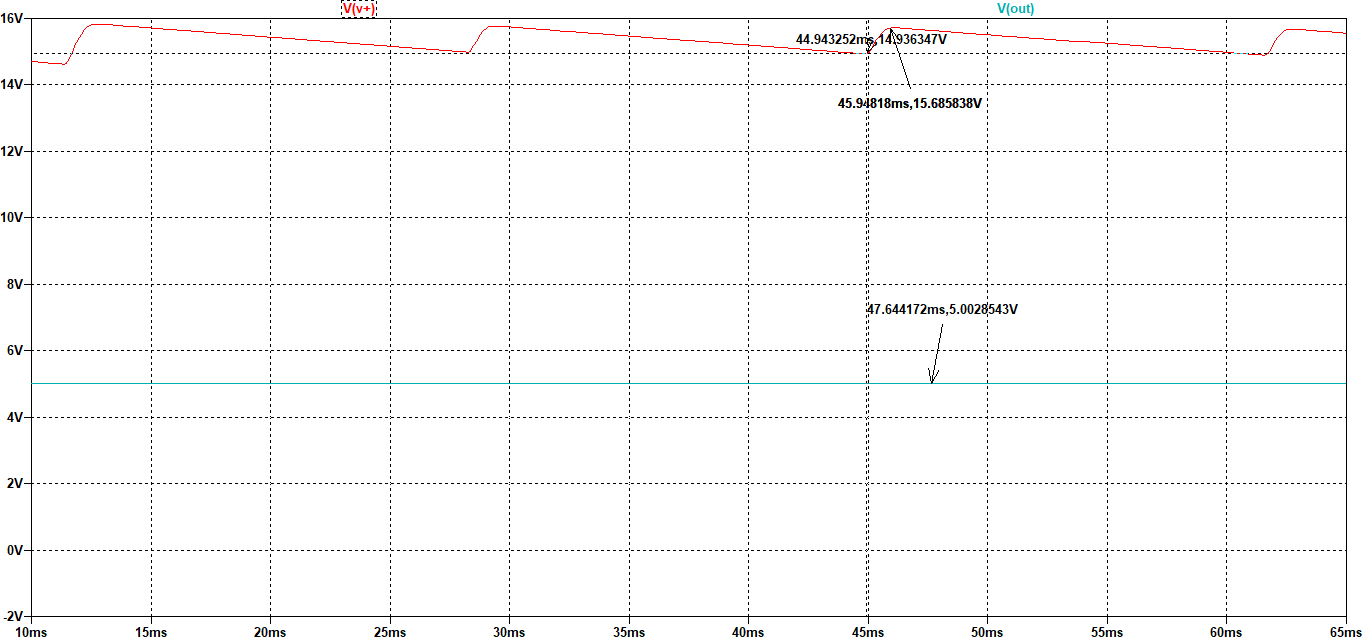
\includegraphics[width=15cm]{Imagenes/sim_reg_sinct_rl2.png}
                                \caption{Voltaje de salida del regulador (V(out)), Voltaje de salida del puente de diodos junto al rizado (V(v+)) con una carga de 240 ohms, dando un voltaje de rizado de 0.768 V}
                                \label{fig:sim_reg_sinct_rl2}
                            \end{figure}

                        \item Simulación de la figura \ref{fig:regulador_sal_ajustable}

                            \begin{itemize}
                                \item Sin Carga
                                    
                                    \begin{figure}[H]
                                        \centering
                                        \renewcommand{\figurename}{Gráfica}
                                        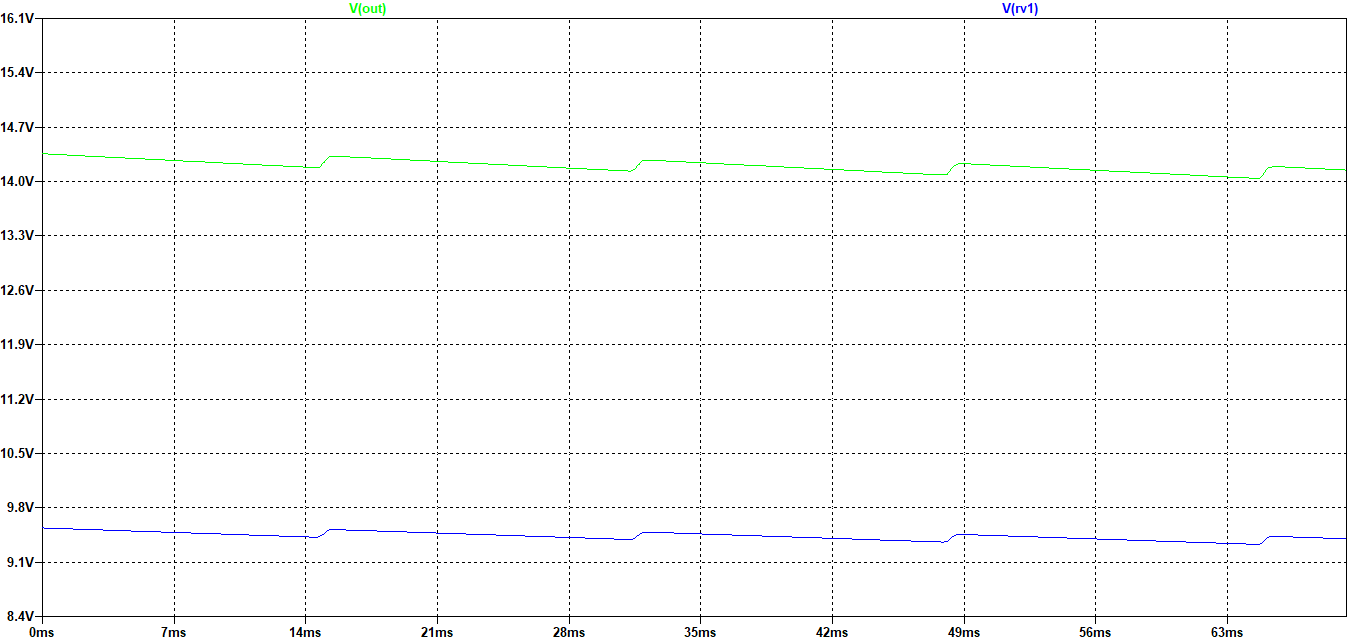
\includegraphics[width=15cm]{Imagenes/sim_regulador_sal_ajustable_sinrl1.png}
                                        \caption{Voltaje de salida del regulador (V(out)), Caída de tensión del potenciómetro en RV1=10k ohm}
                                        \label{fig:sim_regulador_sal_ajustable_sinrl1}
                                    \end{figure}
        
                                    \begin{figure}[H]
                                        \centering
                                        \renewcommand{\figurename}{Gráfica}
                                        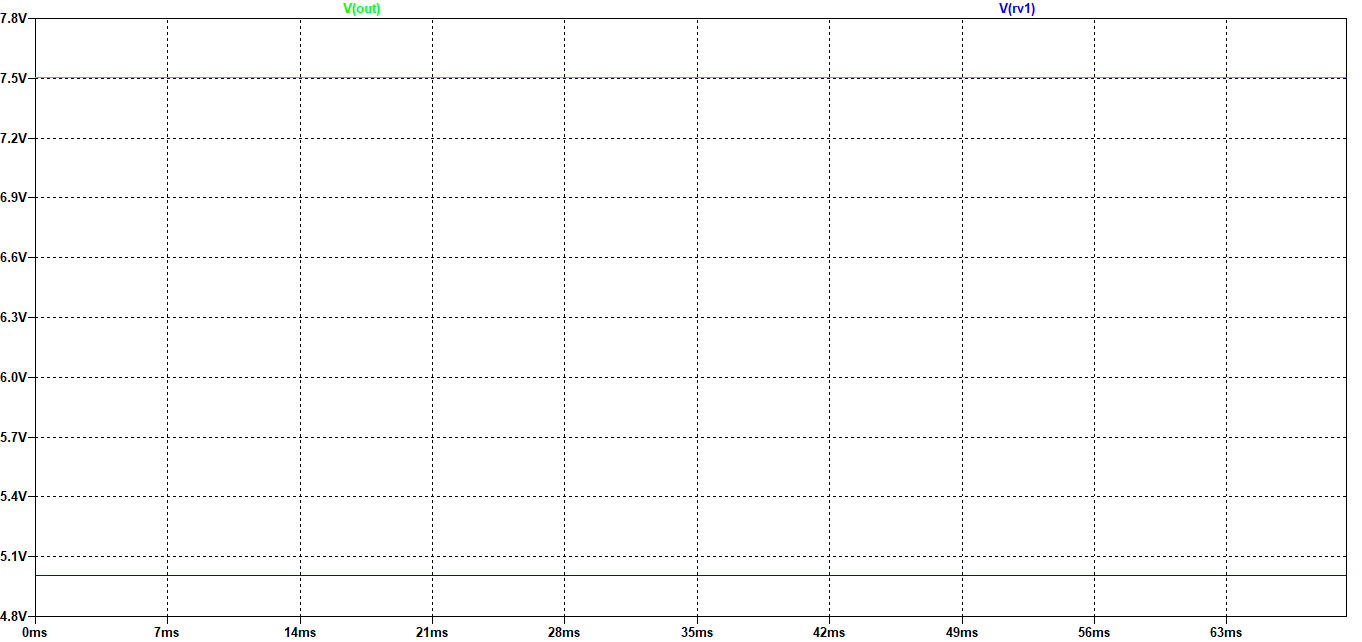
\includegraphics[width=15cm]{Imagenes/sim_regulador_sal_ajustable_sinrl2.png}
                                        \caption{Voltaje de salida del regulador (V(out)), Caída de tensión del potenciómetro en RV1=5k ohm}
                                        \label{fig:sim_regulador_sal_ajustable_sinrl2}
                                    \end{figure}
        
                                    \begin{figure}[H]
                                        \centering
                                        \renewcommand{\figurename}{Gráfica}
                                        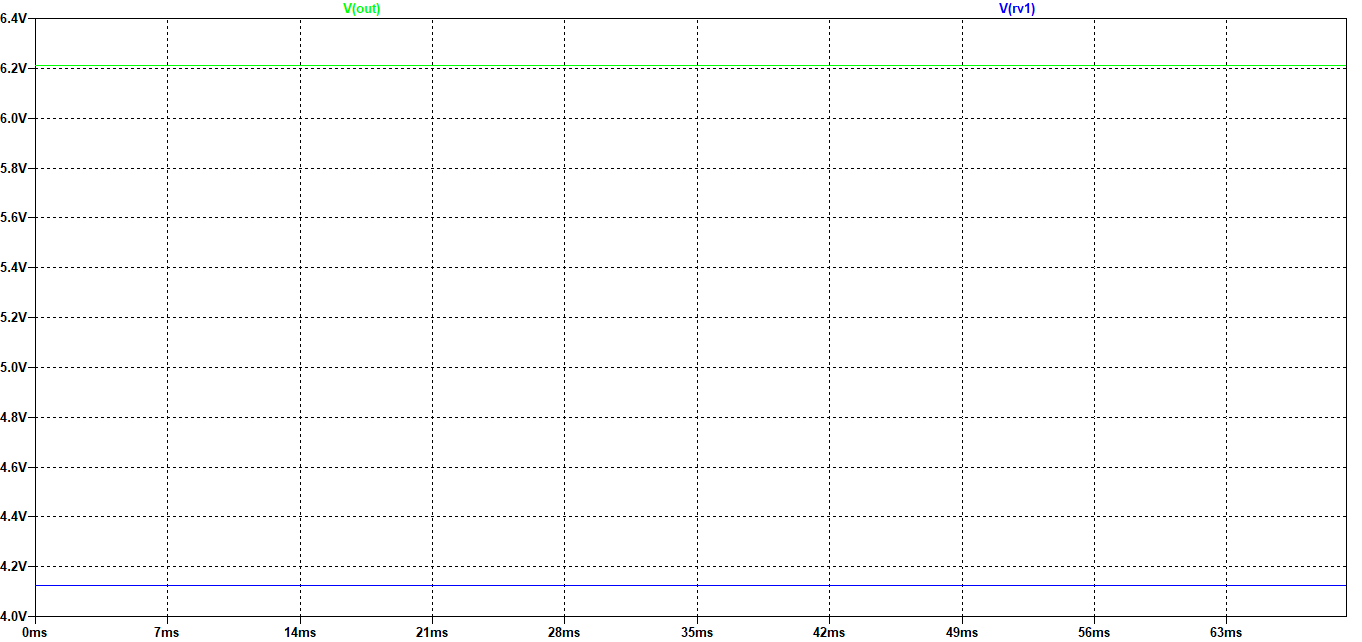
\includegraphics[width=15cm]{Imagenes/sim_regulador_sal_ajustable_sinrl3.png}
                                        \caption{Voltaje de salida del regulador (V(out)), Caída de tensión del potenciómetro en RV1=0.1 ohm}
                                        \label{fig:sim_regulador_sal_ajustable_sinrl3}
                                    \end{figure}
                                    \begin{figure}[H]
                                        \centering
                                        \renewcommand{\figurename}{Gráfica}
                                        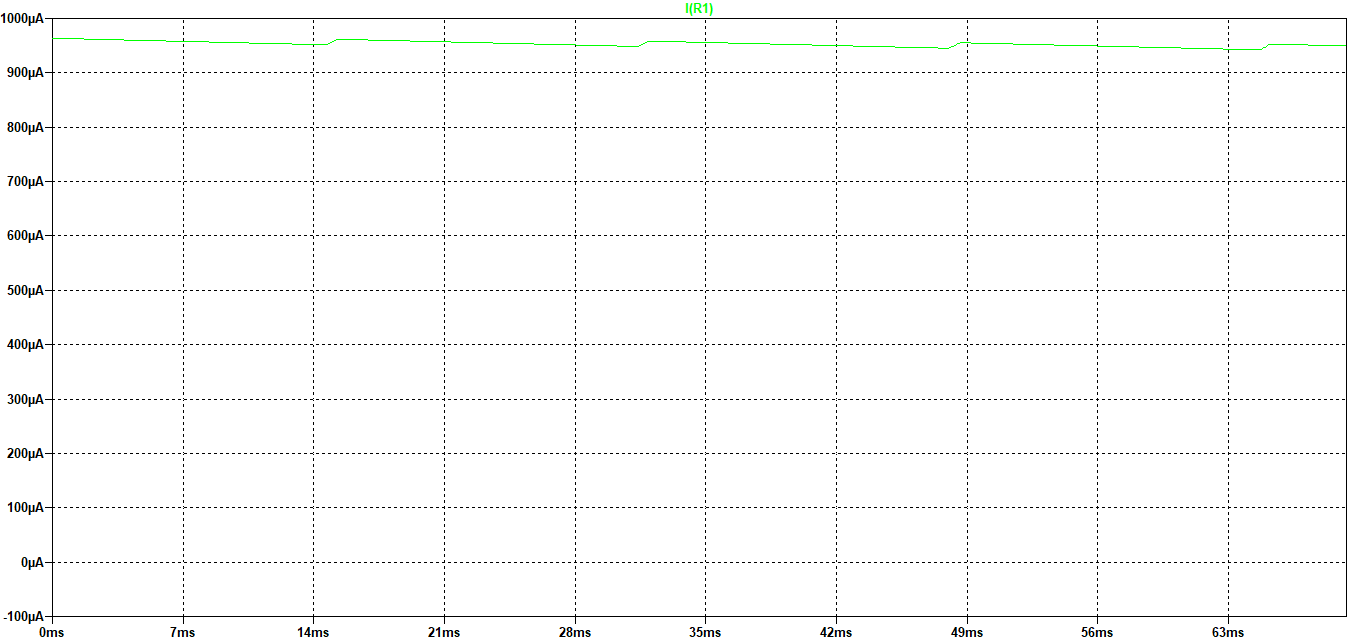
\includegraphics[width=15cm]{Imagenes/sim_regulador_sal_ajustable_corrientesinrl.png}
                                        \caption{Corriente de polarización que suministra el amplificador operacional por la resistencia R1}
                                        \label{fig:sim_regulador_sal_ajustable_corrientesinrl}
                                    \end{figure}
                                    
                                \item Con carga ($R_L=240\ohm$)

                                    \begin{figure}[H]
                                        \centering
                                        \renewcommand{\figurename}{Gráfica}
                                        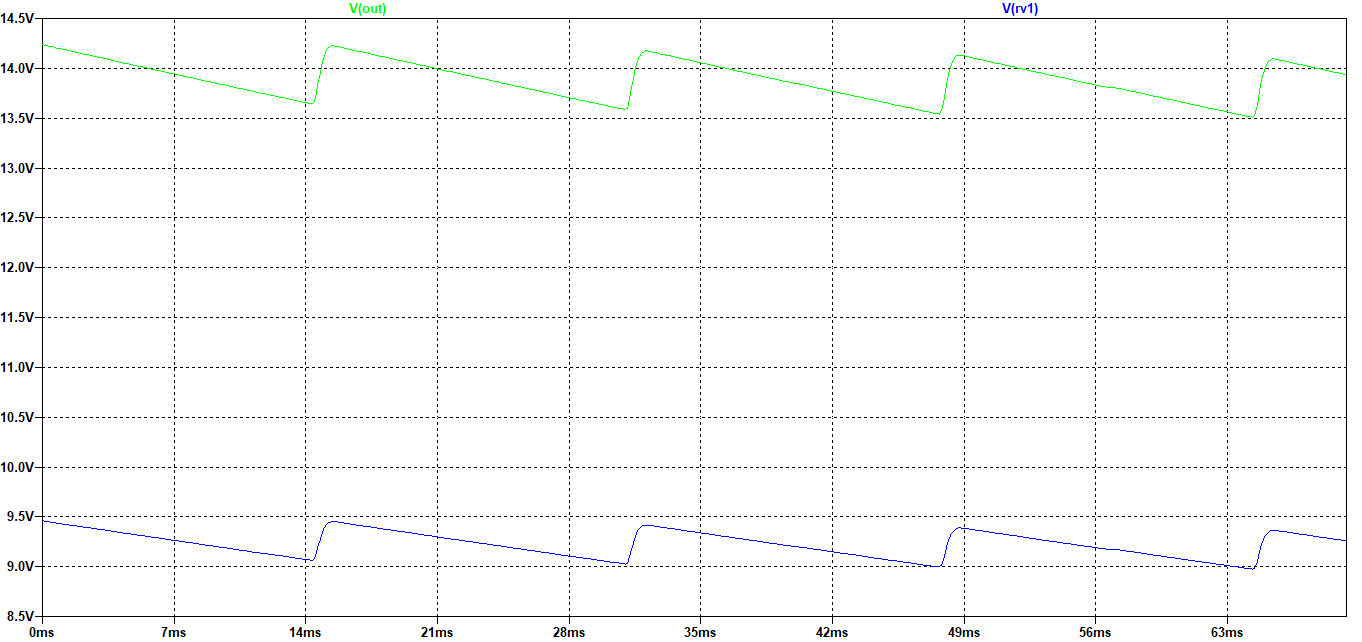
\includegraphics[width=15cm]{Imagenes/sim_regulador_sal_ajustable_conrl1.png}
                                        \caption{Voltaje de salida del regulador (V(out)), Caída de tensión del potenciómetro en RV1=10k ohm}
                                        \label{fig:sim_regulador_sal_ajustable_conrl1}
                                    \end{figure}
        
                                    \begin{figure}[H]
                                        \centering
                                        \renewcommand{\figurename}{Gráfica}
                                        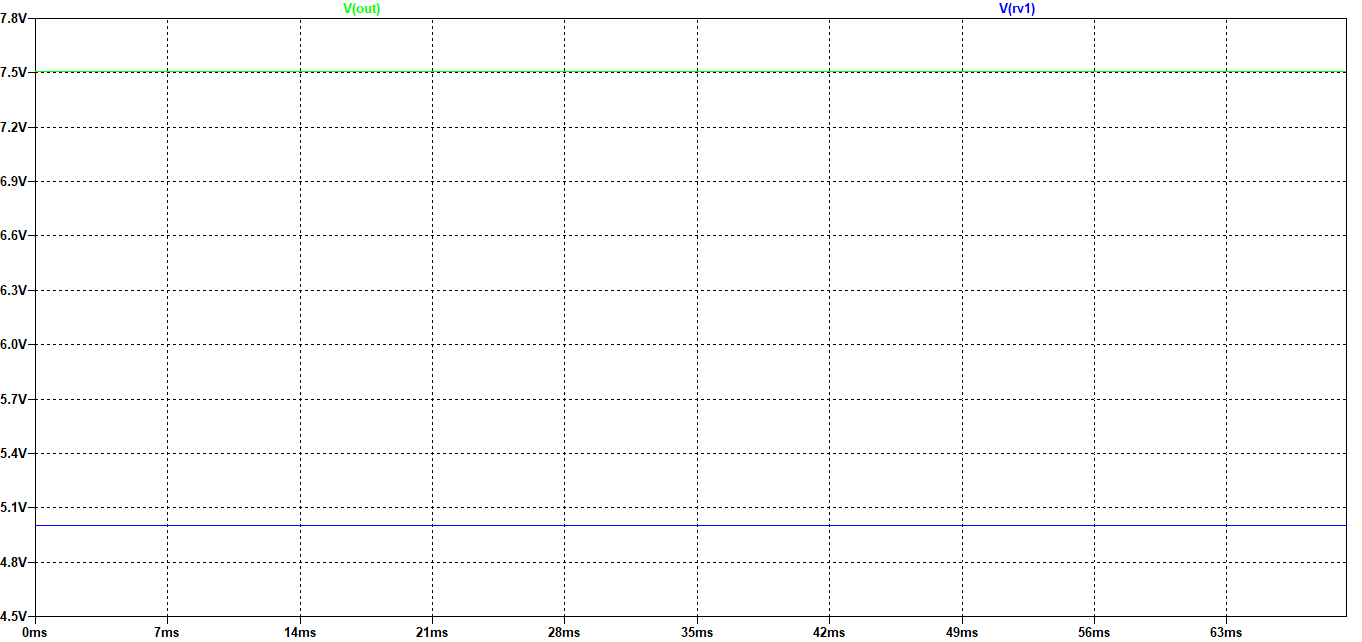
\includegraphics[width=15cm]{Imagenes/sim_regulador_sal_ajustable_conrl2.png}
                                        \caption{Voltaje de salida del regulador (V(out)), Caída de tensión del potenciómetro en RV1=5k ohm}
                                        \label{fig:sim_regulador_sal_ajustable_conrl2}
                                    \end{figure}
        
                                    \begin{figure}[H]
                                        \centering
                                        \renewcommand{\figurename}{Gráfica}
                                        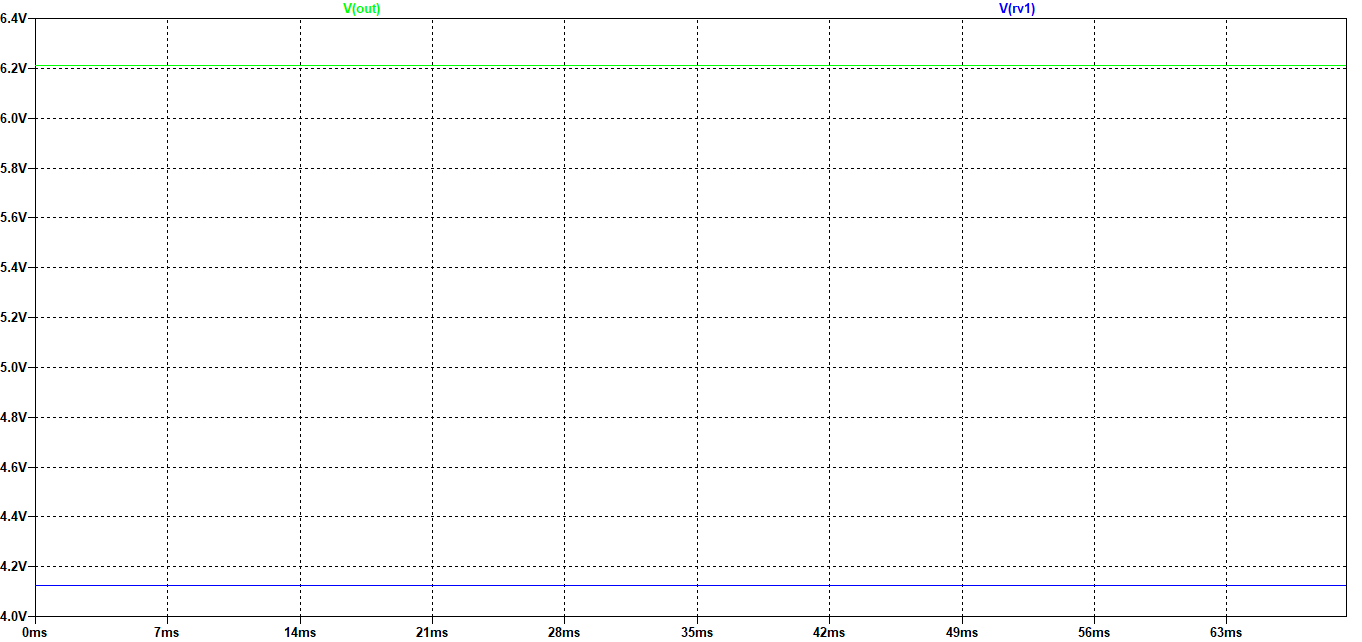
\includegraphics[width=15cm]{Imagenes/sim_regulador_sal_ajustable_conrl3.png}
                                        \caption{Voltaje de salida del regulador (V(out)), Caída de tensión del potenciómetro en RV1=0.1 ohm}
                                        \label{fig:sim_regulador_sal_ajustable_conrl3}
                                    \end{figure}
                                        
                                Como se puede observar en estas simulaciones con carga y sin carga, no existe una variación en su salida, por lo tanto mantiene su regulación
                            \end{itemize}

                        \item Figura \ref{fig:fuente_corriente_variable}

                            \begin{figure}[H]
                                \centering
                                \renewcommand{\figurename}{Gráfica}
                                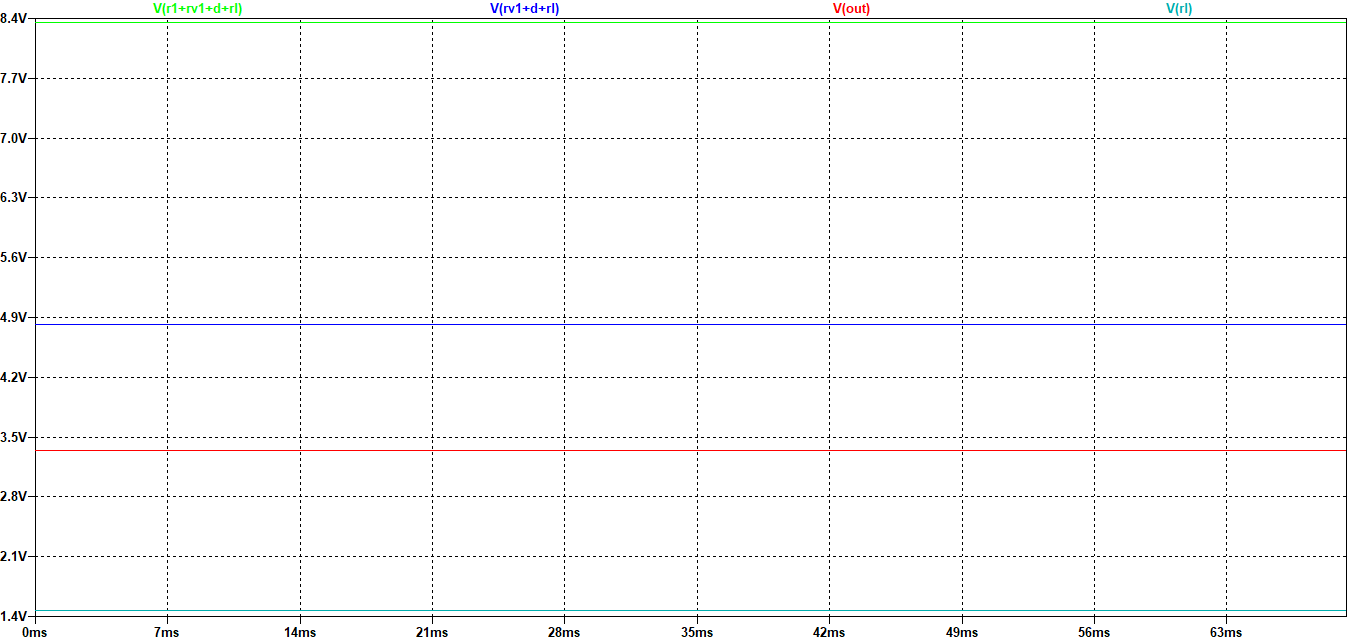
\includegraphics[width=15cm]{Imagenes/sim_fuente_corriente_variable_x01.png}
                                \caption{Caídas de tensión en las distintas cargas y resistencias cuando xRV1=0.1(1k)}
                                \label{fig:sim_fuente_corriente_variable_x01}
                            \end{figure}

                            \begin{figure}[H]
                                \centering
                                \renewcommand{\figurename}{Gráfica}
                                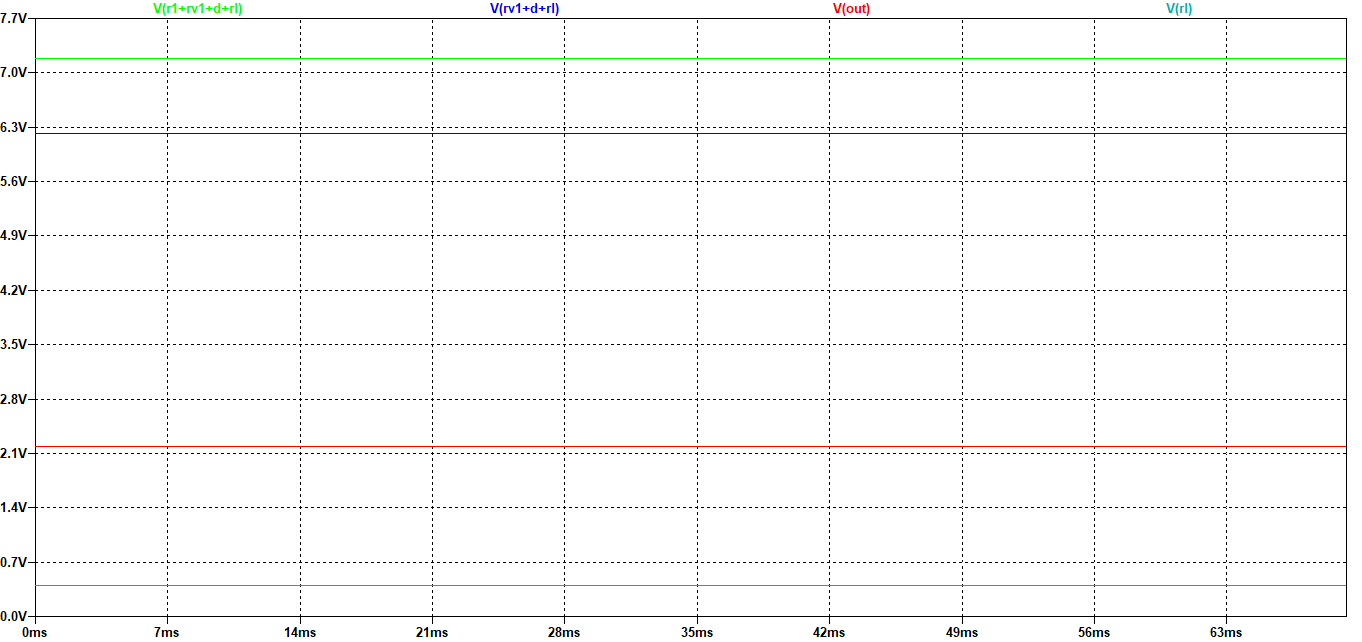
\includegraphics[width=15cm]{Imagenes/sim_fuente_corriente_variable_x1.png}
                                \caption{Caídas de tensión en las distintas cargas y resistencias cuando xRV1=1(1k)}
                                \label{fig:sim_fuente_corriente_variable_x1}
                            \end{figure}

                            \begin{figure}[H]
                                \centering
                                \renewcommand{\figurename}{Gráfica}
                                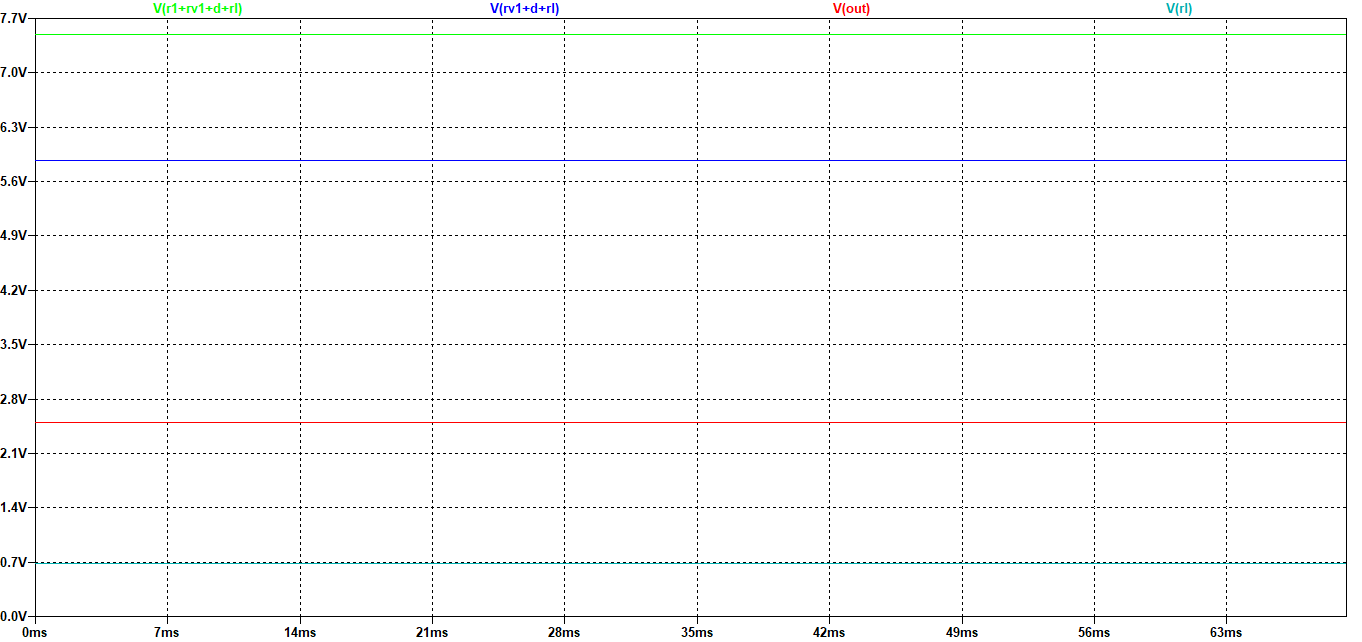
\includegraphics[width=15cm]{Imagenes/sim_fuente_corriente_variable_x05.png}
                                \caption{Caídas de tensión en las distintas cargas y resistencias cuando xRV1=0.5(1k)}
                                \label{fig:sim_fuente_corriente_variable_x05}
                            \end{figure}

                            \begin{figure}[H]
                                \centering
                                \renewcommand{\figurename}{Gráfica}
                                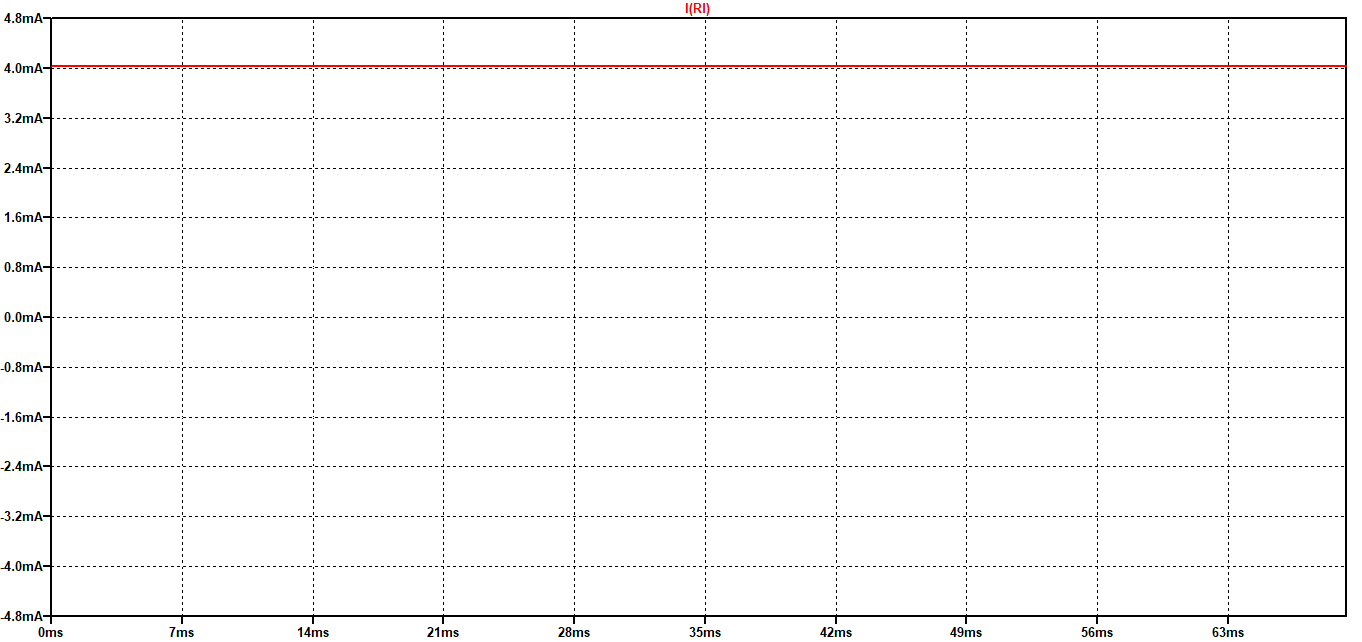
\includegraphics[width=15cm]{Imagenes/sim_fuente_corriente_variable_corrx1.png}
                                \caption{Corriente de salida cuando  xRV1=1(1k)}
                                \label{fig:sim_fuente_corriente_variable_corrx1}
                            \end{figure}

                            \begin{figure}[H]
                                \centering
                                \renewcommand{\figurename}{Gráfica}
                                \includegraphics[width=15cm]{Imagenes/sim_fuente_corriente_variable_corrx01.png}
                                \caption{Corriente de salida cuando  xRV1=0.1(1k)}
                                \label{fig:sim_fuente_corriente_variable_corrx01}
                            \end{figure}

                            \begin{figure}[H]
                                \centering
                                \renewcommand{\figurename}{Gráfica}
                                \includegraphics[width=15cm]{Imagenes/sim_fuente_corriente_variable_corrx05.png}
                                \caption{Corriente de salida cuando  xRV1=0.5(1k)}
                                \label{fig:sim_fuente_corriente_variable_corrx05}
                            \end{figure}

                            
                    \end{itemize}
            \end{enumerate}
        
    \end{enumerate}
    
    Como se observa, los cálculos son los adecuados para la practica, debido a la verificación realizada por cada una de las simulaciones.
\newpage

